\documentclass[11pt]{article}
\usepackage[utf8]{inputenc}
\usepackage{amsthm}
\usepackage{amsmath}
\usepackage{amsfonts}
\usepackage{mathrsfs}
\usepackage{geometry}
\usepackage{graphicx}
\usepackage{bbding}
\usepackage{bm}
\usepackage{xcolor} 
% \usepackage[numbers, sort&compress]{natbib}
\usepackage{natbib}
\usepackage{caption}
\usepackage{subcaption}
\usepackage{algorithm, algpseudocode}
\usepackage{enumitem}

\newcommand{\red}{\color{red}}
\newcommand{\bb}{\color{black}}
\newcommand{\valpha}{\bm{\alpha}}
\newcommand{\vw}{\bm{w}}
\newcommand{\vy}{\bm{y}}
\newcommand{\vr}{\bm{r}}
\newcommand{\vtheta}{\bm{\theta}}
\newcommand{\normtwo}[1]{\left\lVert#1\right\rVert_2}


\theoremstyle{definition}
\newtheorem{definition}{Definition}[section]

\title{Neuronized Priors Project}
\author{Chistopher Crabtree, Lanxin Yang, Yunshan  Duan}
%\date{October 2021}

\begin{document}

\maketitle



% \Huge{\textbf{Report}}
% \normalsize
% \begin{enumerate}
%     \item Intro: Yunshan \checkmark
%     \item Neuronized Prior def.: Yunshan \checkmark
%     \item Neuronization Standard sparse priors
%     \begin{enumerate}
    
%         \item Standard sparse priors
%             \begin{enumerate}
%                 \item SpSl: Yunshan \checkmark
%                 \item Bayesian Lasso: Chris\checkmark 
%                 \item HS, Cauchy: Lanxin\checkmark
%             \end{enumerate}
%         \item Neuronization
%             \begin{enumerate}
%                 \item SpSl: Yunshan \checkmark
%                 \item Bayesian Lasso: Chris \checkmark
%                 \item HS, Cauchy: Lanxin\checkmark
%                 \item How to find neuronized priors: Lanxin\checkmark
%             \end{enumerate}
%     \end{enumerate}
%     \item Sampling/Optim.: Yunshan \checkmark
%     \item Theory: Chris
%     \item Simulation: 
%     \begin{enumerate}
%         \item Synthetic data: Yunshan \checkmark
%         \item Metrics : Chris \checkmark
%         \item Analysis: Yunshan \checkmark
%     \end{enumerate}
%     \item Real data: Chris \checkmark
%     \item Conclusion: Lanxin
% \end{enumerate}

% \Huge{\textbf{Video}}
% \normalsize
% \begin{enumerate}
%     \item Lanxing: 1. Intro, 2.Neronized Prior def., and 3.a Standard sparse priors
%     \item Yunshan: 3.b Neuronization, 4. Sampling/Optim, 5.Theory? 
%     \item Chris: 6. Simulation, 7. Real data, 8.Conclusion
% \end{enumerate}

\begin{abstract}
  This paper presents a description and replication of the primary results of ``Neuronized Priors for Bayesian Sparse Linear Regression'' by Minsuk Shin and Jun S. Liu. We implemented the MCMC sampling algorithm and the MAP optimization algorithm for the neuronized priors proposed in this paper. And we also implemented the methods of their standard shrinkage prior counterparts, including the SpSL, Bayesian LASSO, and horseshoe priors. Simulation studies and real data examples are investigated, and comparison between optimization methods are conducted. The results are parallel to those in the original paper, that neuronized priors yields similar performance as the standard shrinkage priors, and have computational advantage by reducing the complexity when sampling from the posteriors.
\end{abstract}

\section{Introduction}

Consider the standard linear regression model
$$ \bm{y} = X \bm{\theta} + \bm{\epsilon}, $$
where $\bm{\epsilon} \sim N(0,\sigma^2 I)$. $\bm{y} = (y_1, \dots, y_n)^T $ is the vector of responses, $X$ is the $n \times p$ covariate matrix, $ \bm{\theta} = (\theta_1, \dots, \theta_p)^T \in \mathbb{R}^p$ is the coefficient vector.

To assume sparsity on the prior of $\bm{\theta}$, a shrinkage prior is often imposed on $\theta_j$'s. One popular class of shrinkage prior is the one-group continuous shrinkage prior, which is a hierarchical scale-mixture of Gaussian distributions. 
$$ \theta_j | \nu_w^2, \tau_j^2 \sim N(0,\nu_w^2\tau_j^2),$$
where $\tau_j^2 \sim \pi_\tau$ and $\nu_w  \sim \pi_g$ are pre-specified.
A few choices of the distributions have been shown in induce desirable shrinkage, including the Strawderman-Berger prior, the \textbf{Bayesian Lasso} \citep{park2008bayesian}, the \textbf{horseshoe} prior \citep{carvalho2010horseshoe}, the generalized double Pareto, and the Dirichlet-Laplace prior.

Another popular class pf shrinkage prior is the \textbf{spike-and-slab (SpSL)} priors \citep{mitchell1988bayesian,george1993variable}, also known as two-group mixture priors. It can be written as a mixture of the ``spike'' distribution $\pi_0$, highly concerntrated around zero, and the ``slab'' distribution $\pi_1$, which is relatively disperse.

The paper \citep{shin2021neuronized} proposes \textbf{neuronized priors}, in which each regression coefficient is reparameterized as a product of a weight parameter and a transformed scale parameter via an activation function. Popular shrinkage priors fit this unified form of neuronized priors, including SpSL, Bayesian Lasso, Cauchy, horseshoe, ect.

It is demonstrated in \cite{shin2021neuronized} that the variable selection procedures based on the neuronized priors have the advantage both computationally and theoretically. The characteristic of unifying various classes of shrinkage priors allow one to test out different priors simply by changing the activation function. Additionally, posterior inference of neuronized priors does not rely on the prior-likelihood conjugacy, leading to comparable or better efficiency in computation compared to the standard priors. Moreover, with the conditions put on the activation function and the hyperpriors, the neuronized Bayesian regression achieves the optimal posterior contraction rate and the RWMH algorithm converges to the target distribution at an exponential rate.

The rest part of the paper is organized as follows. Section 2 gives the detailed definition of the neuronized priors. Section 3 shows a few popular shrinkage priors including the SpSL, Bayesian Lasso, horseshoe, and Cauchy priors, and their neuronized counterparts. Section 4 illustrates the computational strategies of posterior inference and the advantages and the neuronized priors. Simulation studies are conducted in Section 5 to compare the results of inference based on different priors and their neuronized counterparts. Two real data examples are also analyzed in Section 5. And conclusions are given in Section 6.



\section{Neuronized prior} \label{sec:neu_def}

\begin{definition}[Neuronized prior]
A neuronized prior is for $\theta_j$ is defined as
\begin{equation} \label{eq:neuronized}
    \theta_j := T(\alpha_j-\alpha_0)w_j,
\end{equation}
where $T$ is a non-decreasing activation function, the scale parameter $\alpha_j$ follows $N(0,1)$, and the weight parameter $w_j$ follows $N(0,\tau_w^2)$, all independently for $j = 1, \dots, p$.
\end{definition}

Under the neuronized prior for $\bm{\theta}$, and the prior $\pi(\sigma^2)$ for $\sigma^2$, the joint posterior distribution can be written as
\begin{align} \label{eq:post_joint}
    \pi(\valpha,\vw, \sigma^2 | \vy, \alpha_0) \propto \frac{\pi(\sigma^2)}{\sigma^n} \exp \{ -\frac{ \normtwo{\vy - X\vtheta(\valpha, \vw, \alpha_0)}^2}{2\sigma^2} -\frac{\valpha^T \valpha}{2} - \frac{\vw^T \vw}{2\tau_w^2} \},
\end{align}
where  $\valpha = \{ \alpha_1, \dots, \alpha_p \}^T$, $\vw = \{w_1, \dots, w_p\}^T$, and 
$$\vtheta (\valpha, \vw, \alpha_0) = \{T(\alpha_1 - \alpha_0)w_1, \dots, T(\alpha_p - \alpha_0)w_p \}^T \mathrel{\widehat{=}} D_{\alpha} \vw,$$
in which $D_\alpha$ is the diagonal matrix with diagonal elements the $T(\alpha_j - \alpha_0)$'s.

\section{Neuronization of Standard Sparse Priors}


\subsection{ Discrete and Continuous SpSL Priors}

The spike-and-slab priors \citep{mitchell1988bayesian,george1993variable} are defined as
\begin{align}
    \theta_j | \gamma_j &\sim (1-\gamma_j) \pi_0(\theta_j) + \gamma_j \pi_1(\theta_j) \\
    \gamma_j &\sim \text{Bernoulli}(\eta) \nonumber
\end{align}

When $\pi_0$ is the point-mass at zero, we call the prior a discrete SpSL prior, otherwise we call it a continuous prior. Typically, $\pi_0$ and $\pi_1$ for a continuous SpSL prior can be defined as two Gaussian distributions with a small and a large variance, respectively.

The computation of the posterior inference based on the discrete SpSL prior is often challenging. Several MCMC sampling strategies and stochastic search strategies have been proposed in literature to counter the difficulty. The MCMC sampling of the posterior using the continuous prior can be more efficiently implemented because of the advantage of conjugacy. However, compared to discrete SpSL prior, the continuous prior does not automatically conclude selected coefficients, and extra variable selection steps are required. 

Let the activation function in Equation \eqref{eq:neuronized} be the rectifier linear unit (ReLU) function,
$$ T(t) = \max \{0,t\}.$$
Set $\alpha_0 = 0$, then the activation function $T(\alpha_j - \alpha_0)$ follows an equal mixture of a point mass at zero and the half standard Gaussian. Under this setting, the neuronized prior in Equation \eqref{eq:neuronized} is equivalent to the discrete SpSL distribution with $\eta=\frac{1}{2}$, which is in the form
\begin{align}
    \theta | \gamma & \sim (1-\gamma) \delta_0(\theta) + \gamma \pi(\theta), \\
    \gamma &\sim \text{Bernoulli} (\frac{1}{2}), \nonumber
\end{align}

Figure \ref{fig:SpSL_prior} shows the histogram of $T(\alpha)$, $T(\alpha)w$, and the standard SpSL prior. Here $\tau_w^2 = 1$. As is shown in the figure, the neuronized prior using the ReLU function as activation function is equivalent to the discrete SpSL prior.

\begin{figure}[t]
     \centering
     \begin{subfigure}[b]{0.49\textwidth}
         \centering
         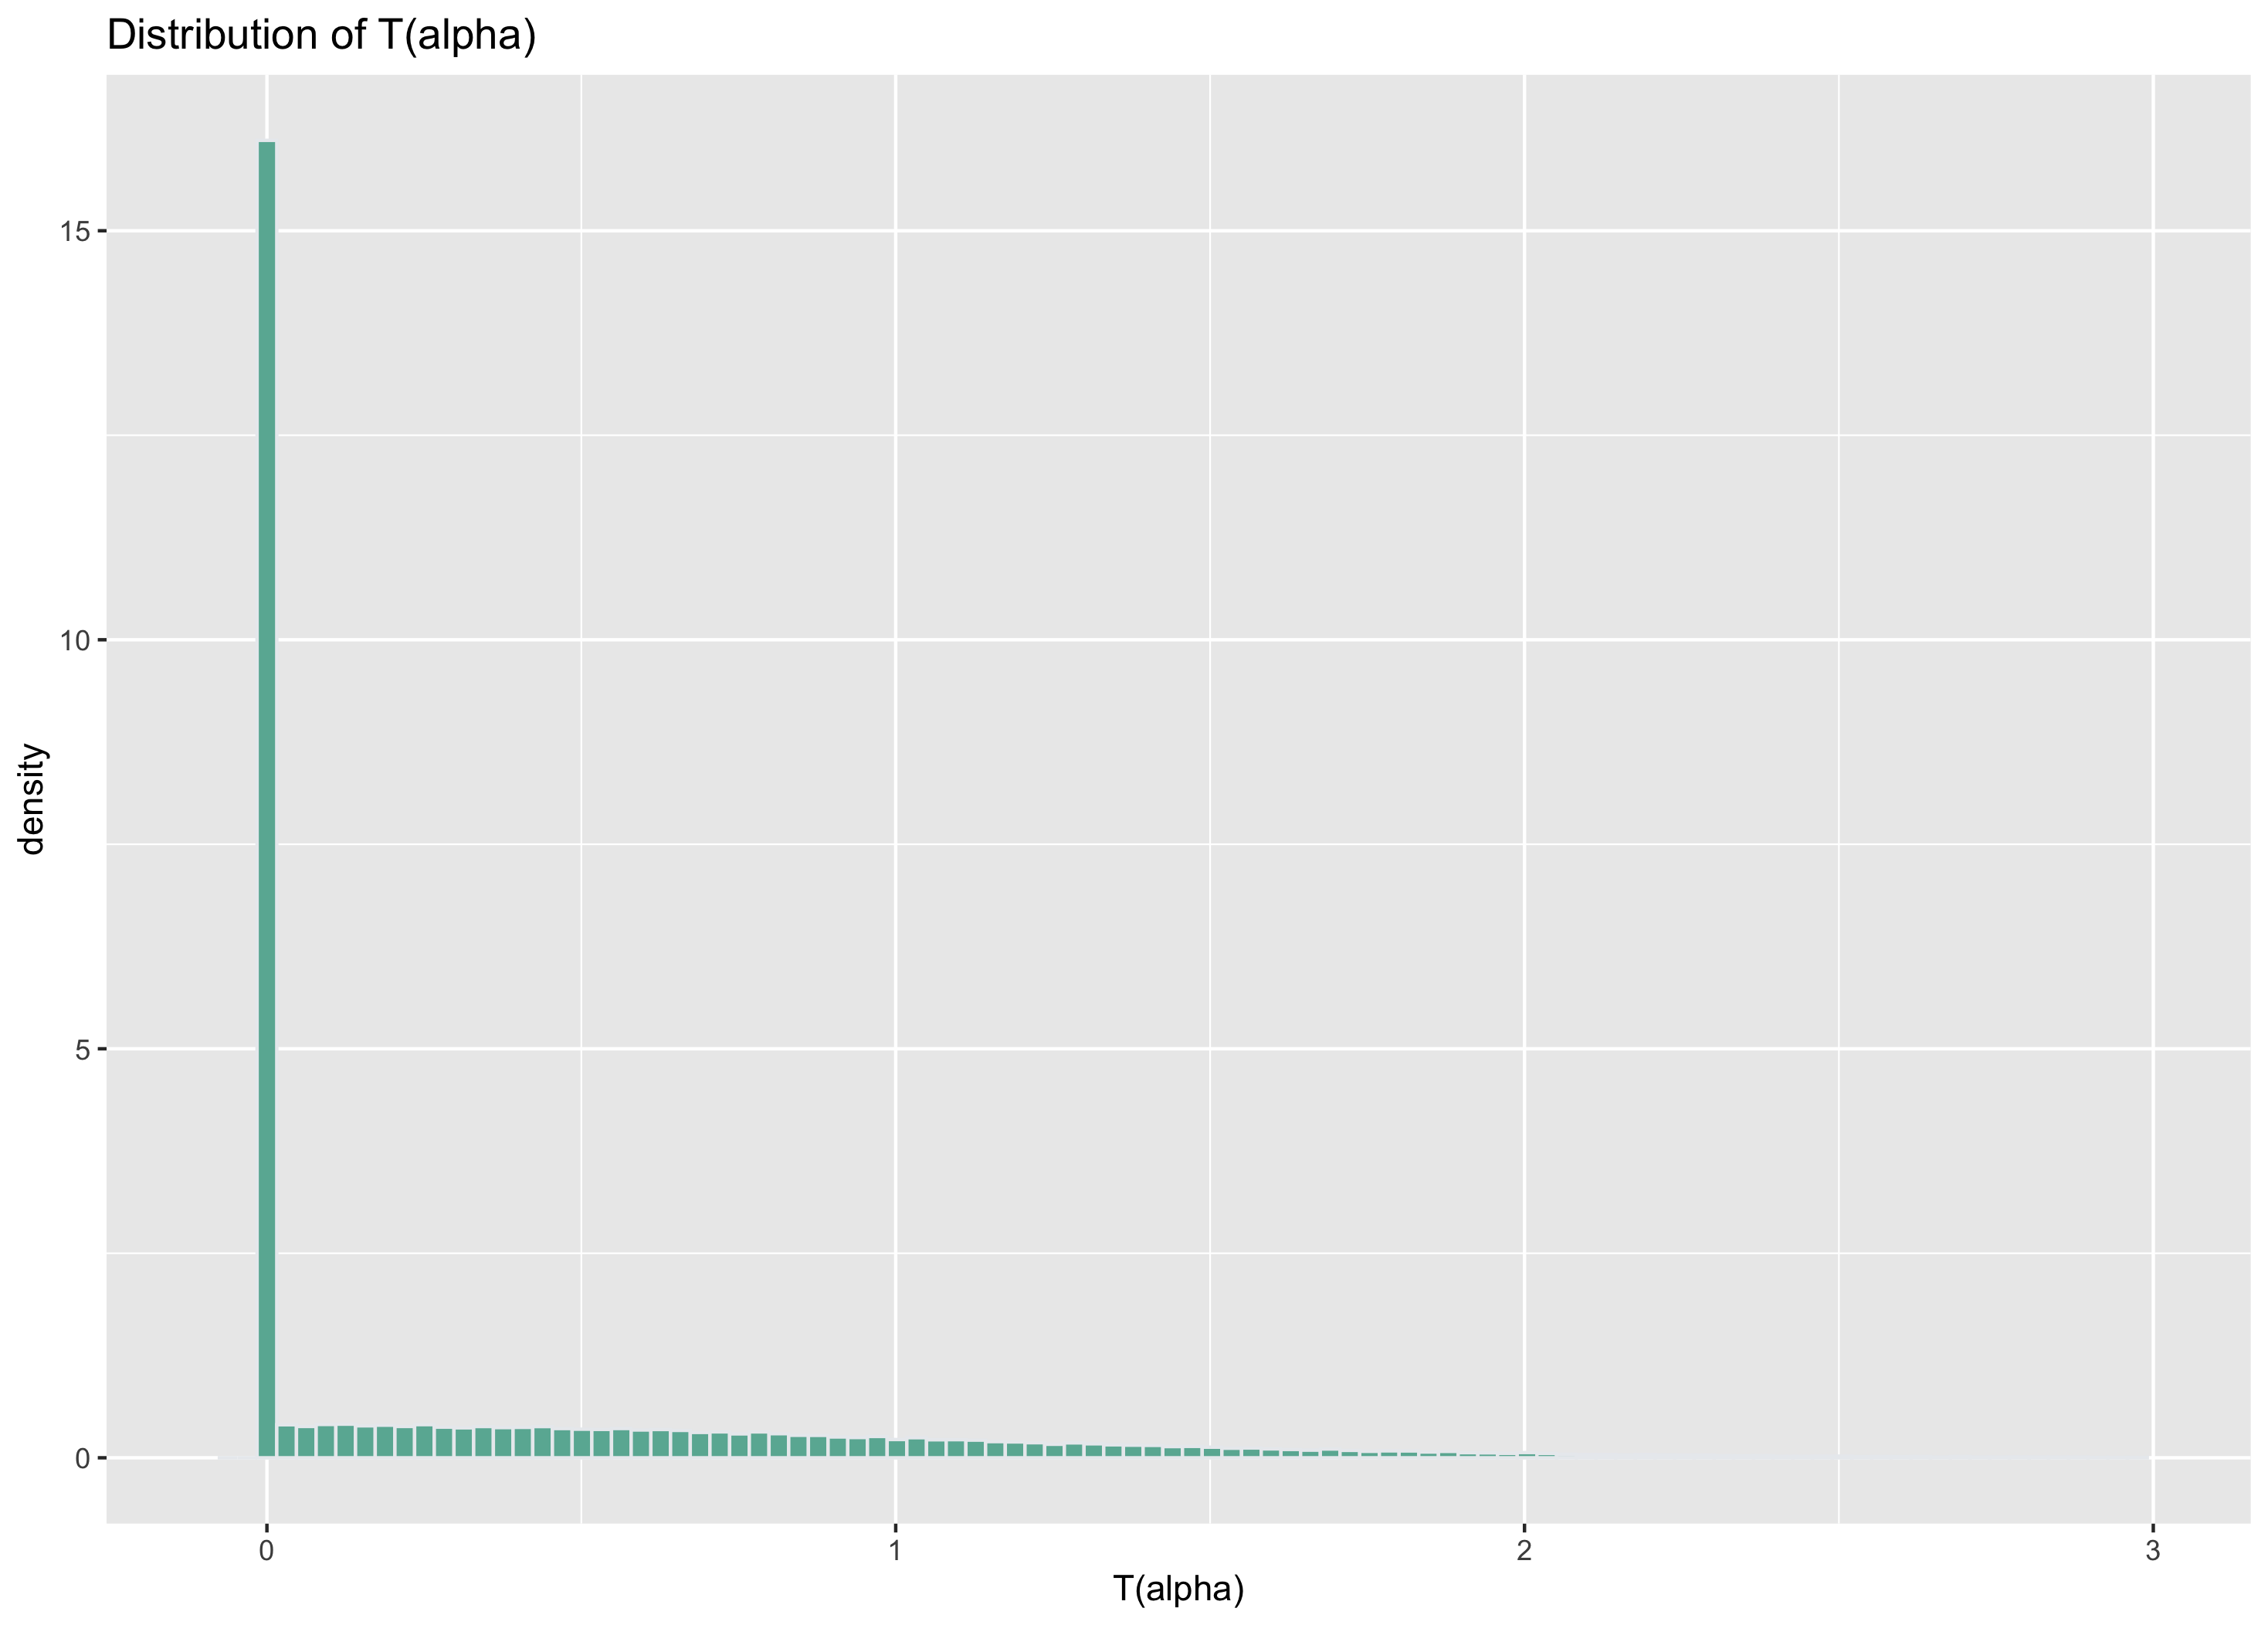
\includegraphics[width=\textwidth]{Figures/SpSLprior1.png}
     \end{subfigure}
     \hfill
     \begin{subfigure}[b]{0.49\textwidth}
         \centering
         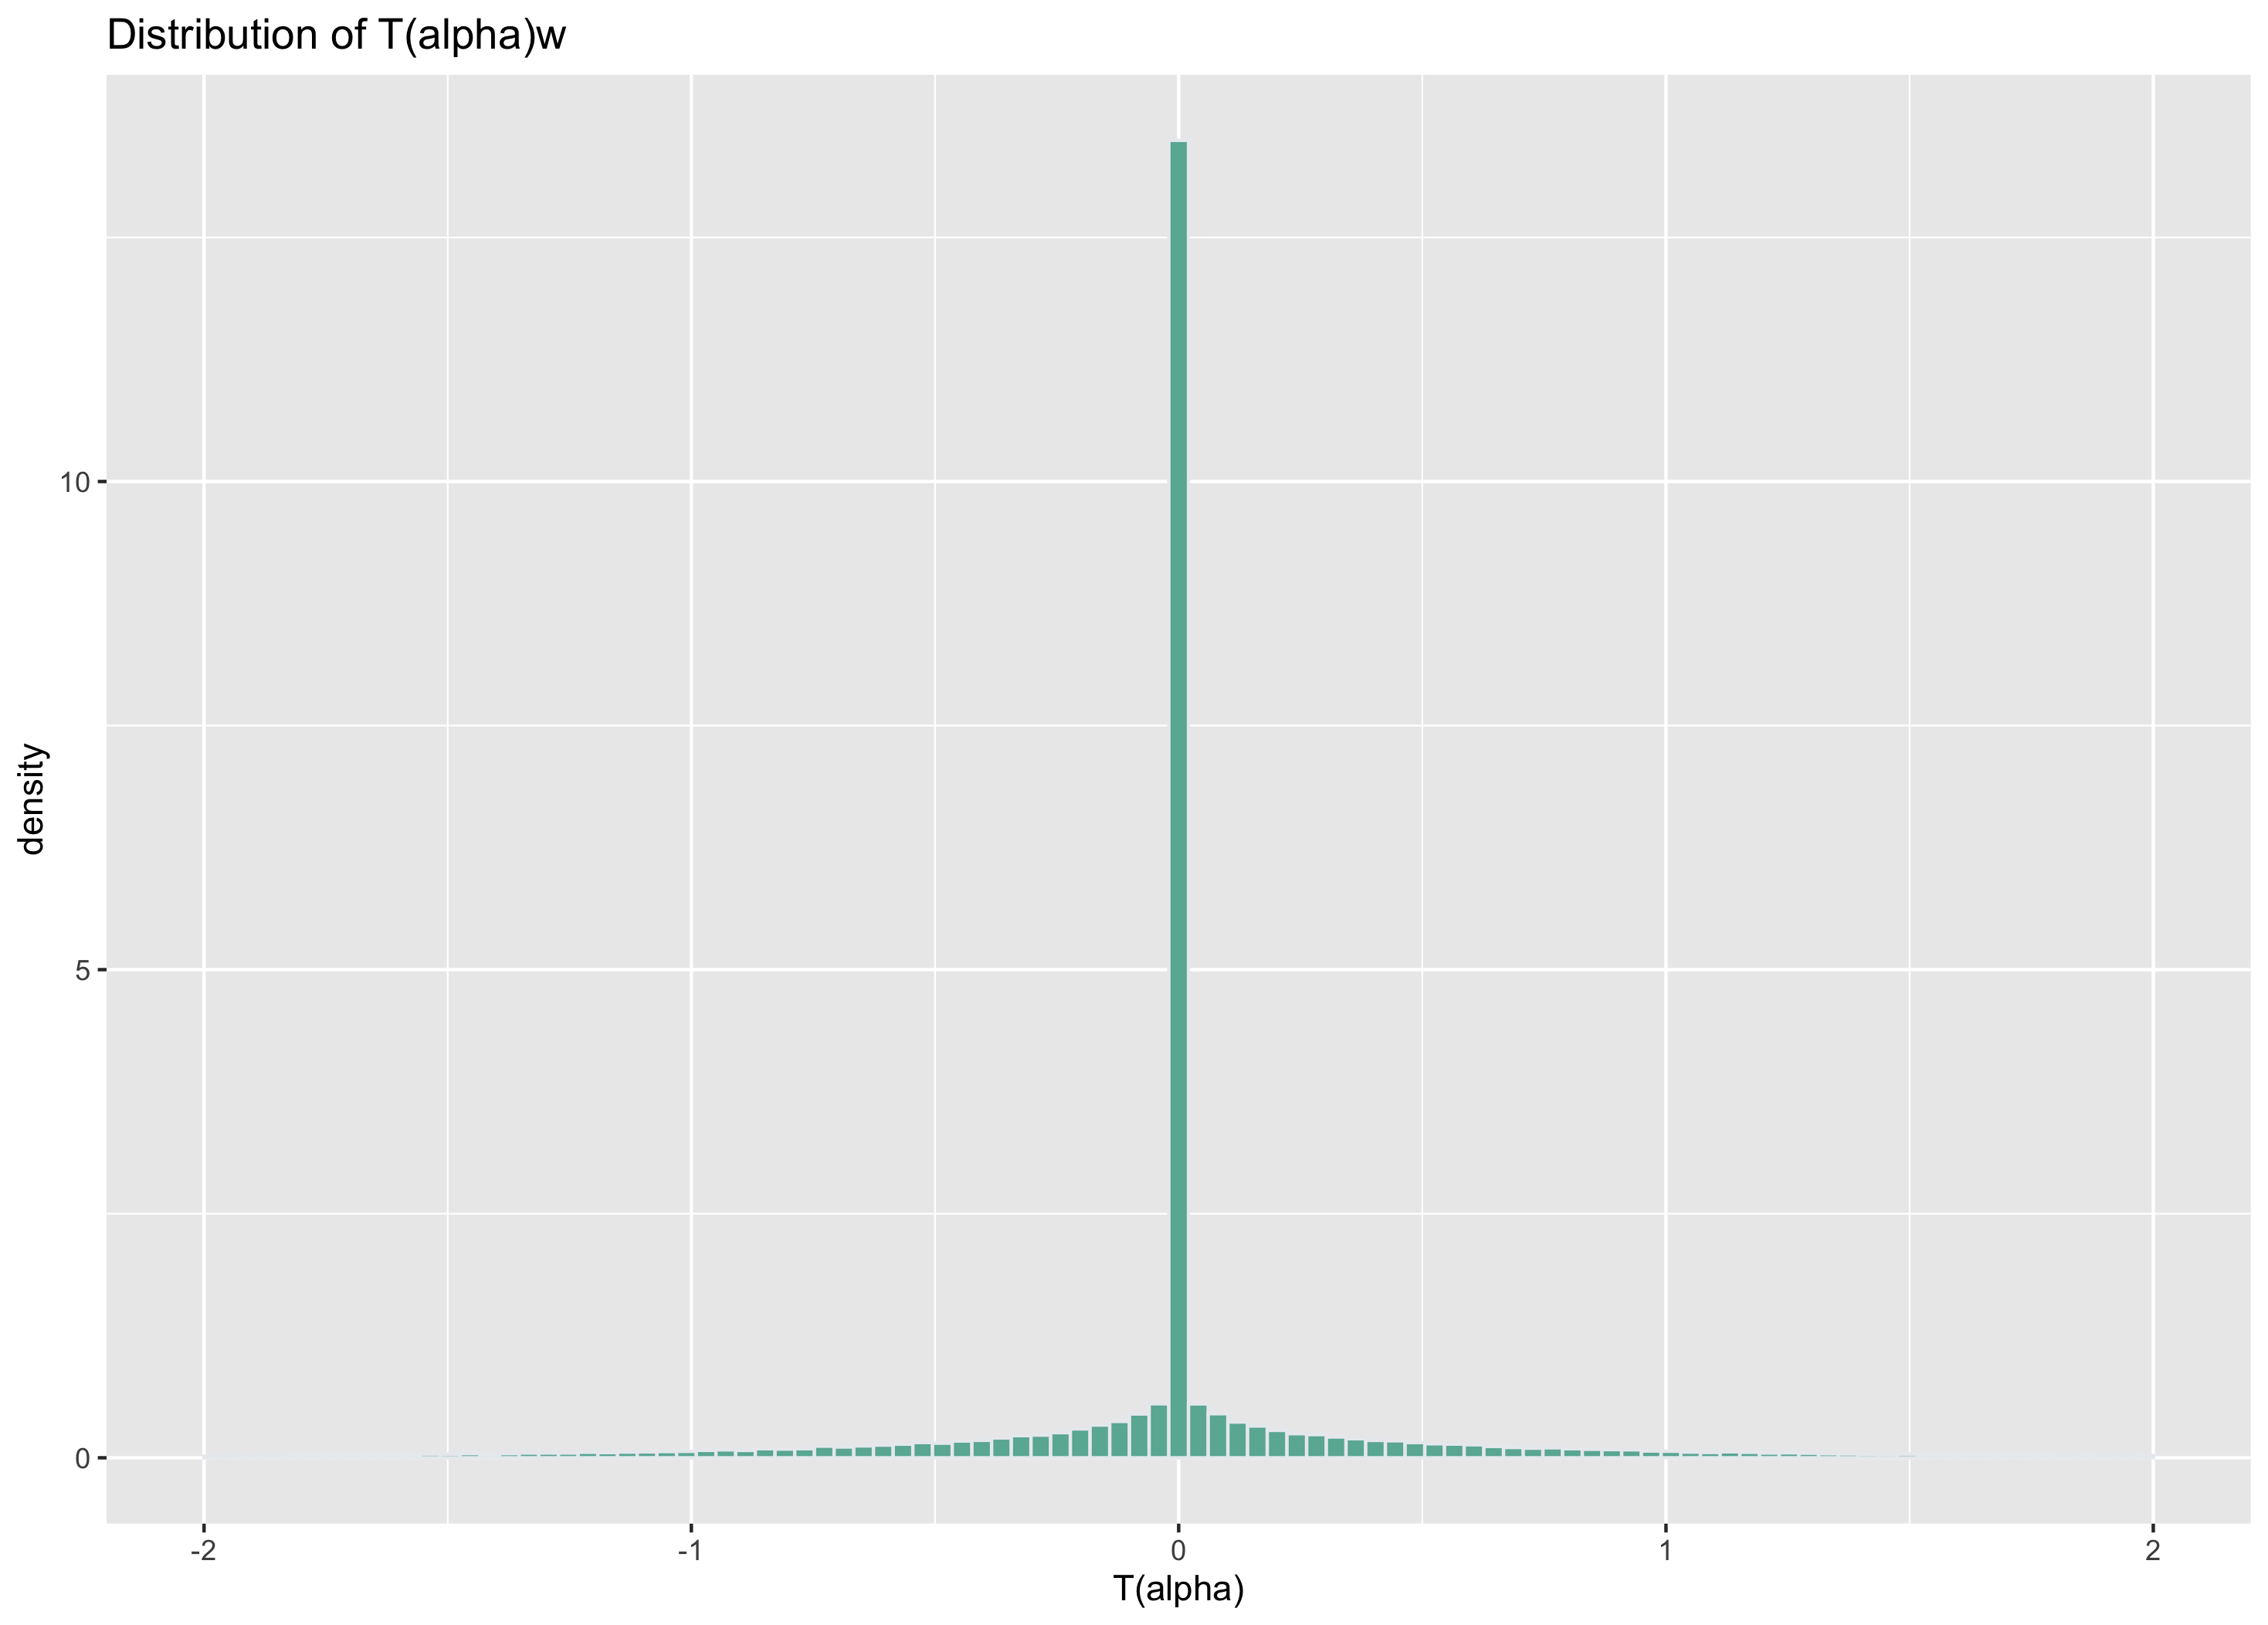
\includegraphics[width=\textwidth]{Figures/SpSLprior2.png}
     \end{subfigure}
     \hfill
     \begin{subfigure}[b]{0.49\textwidth}
         \centering
         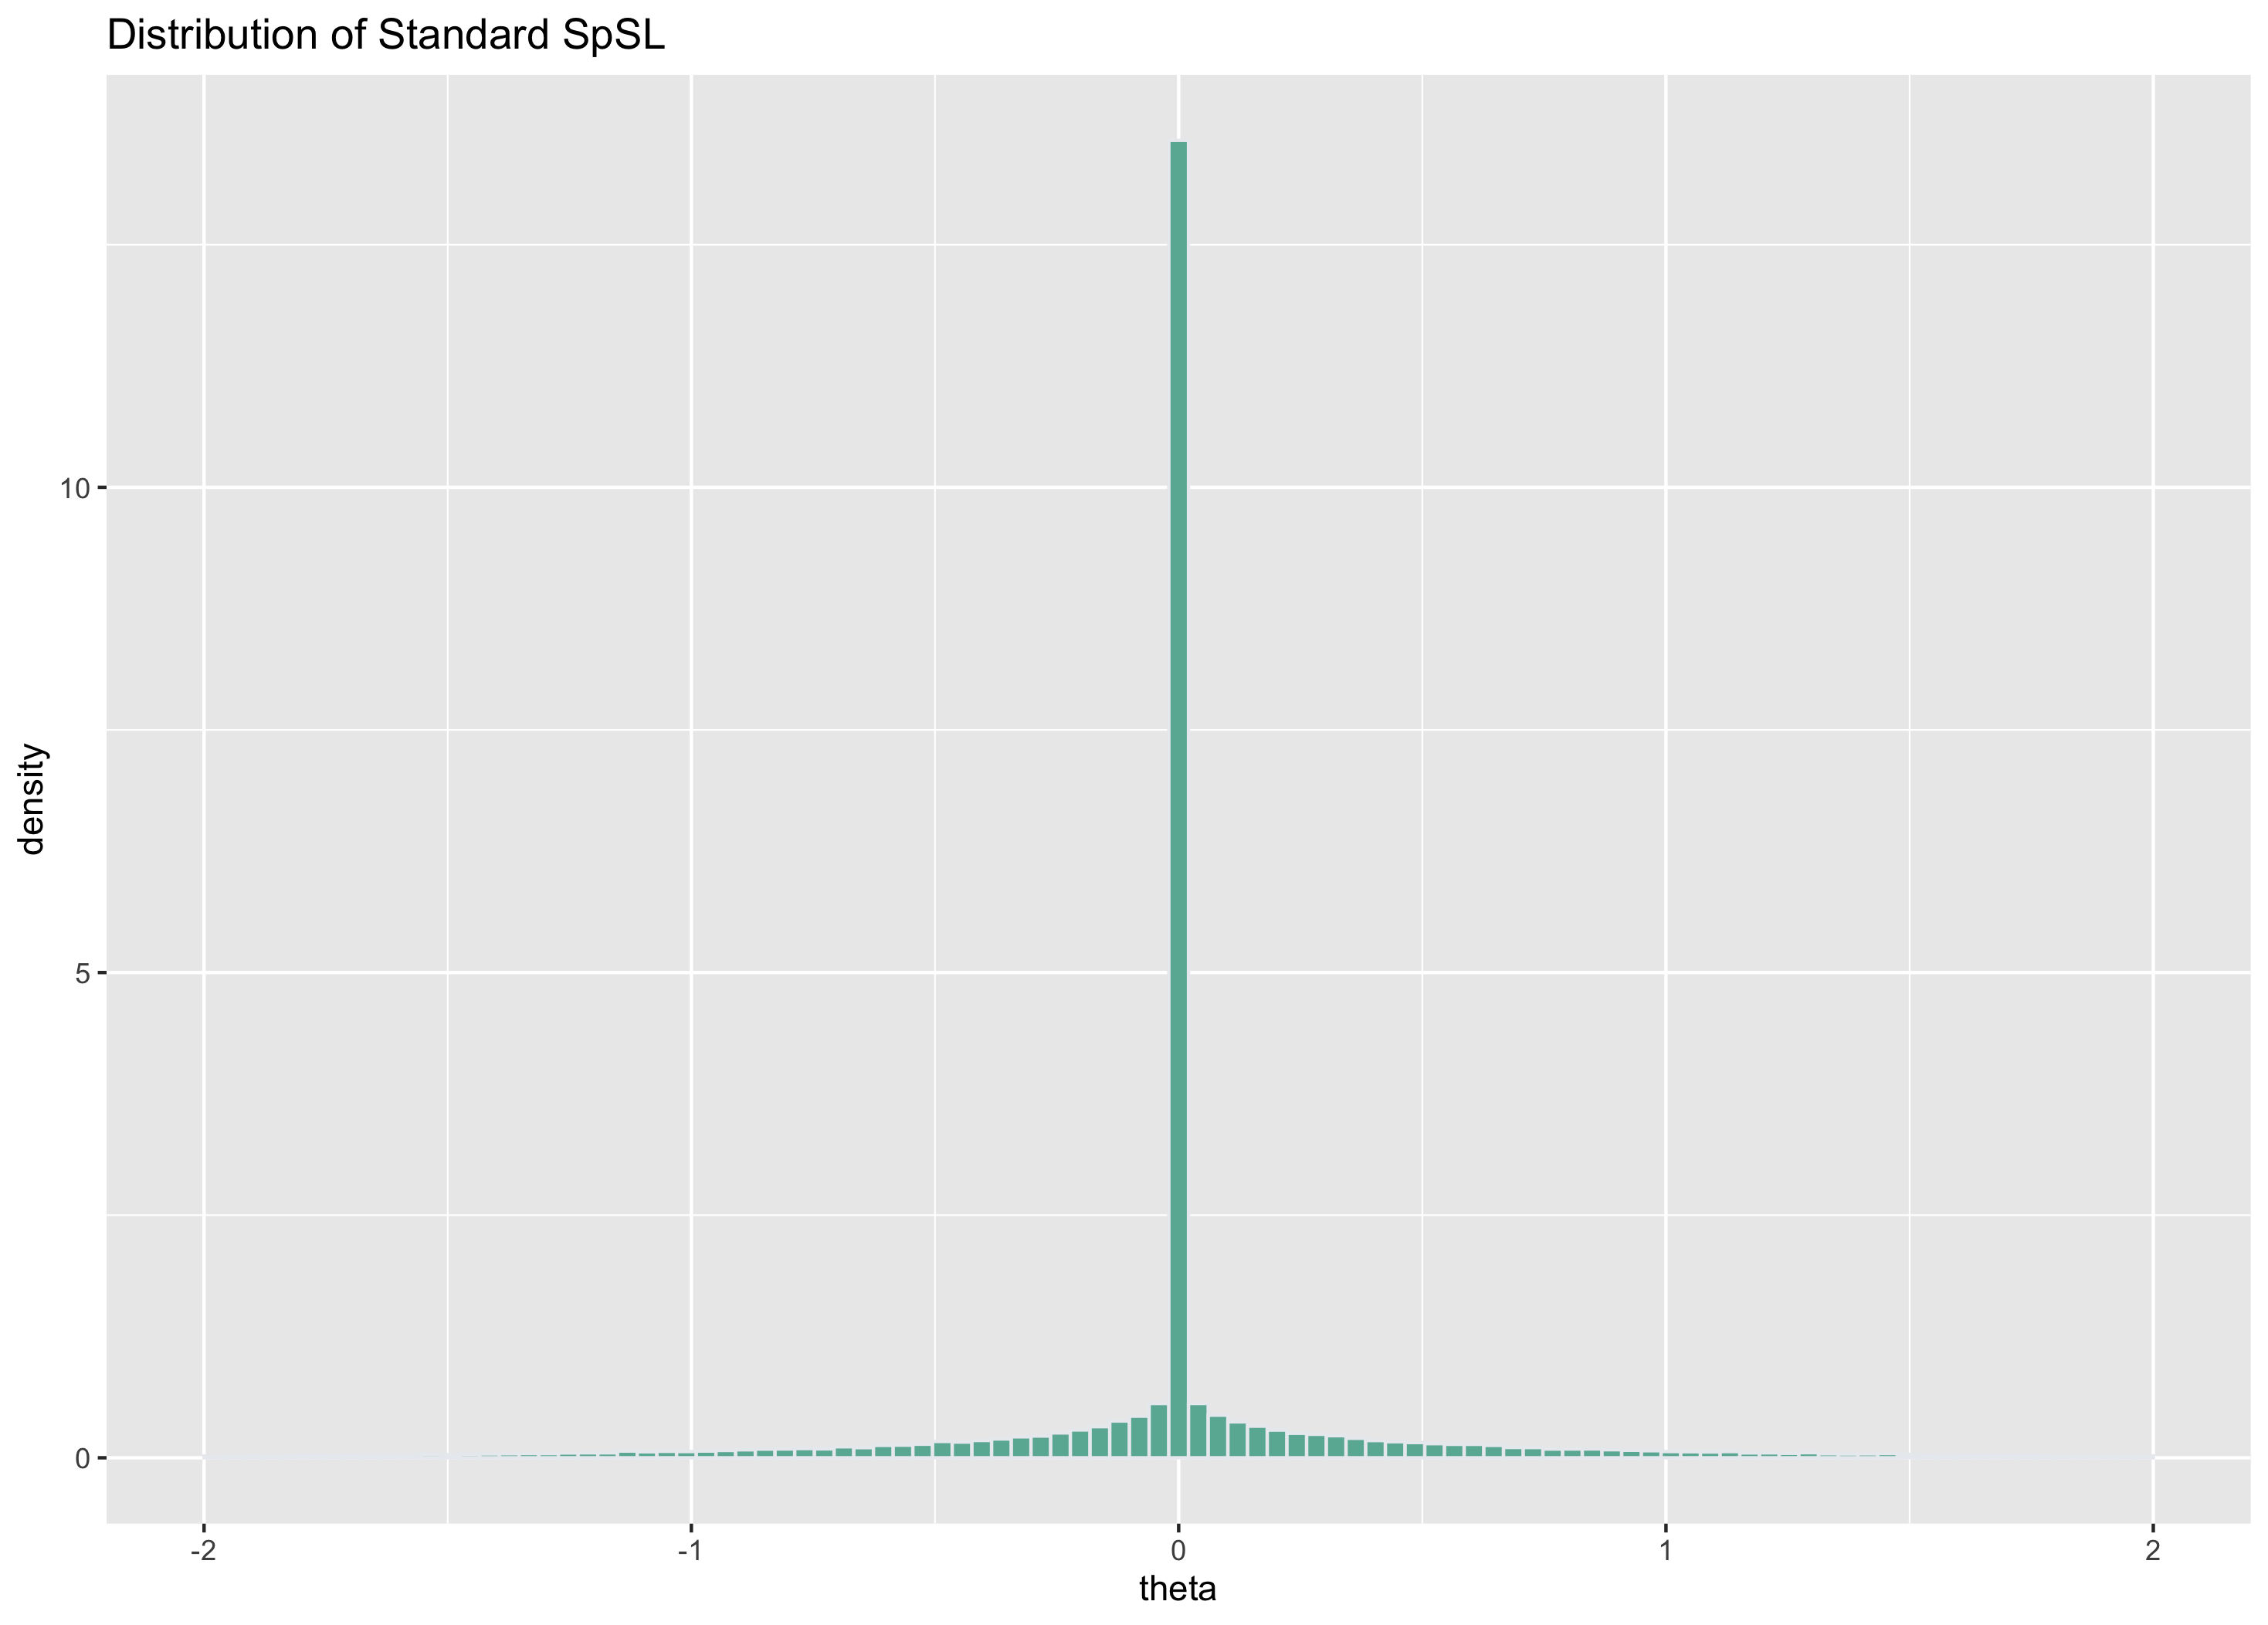
\includegraphics[width=\textwidth]{Figures/SpSLprior3.png}
     \end{subfigure}
        \caption{Histogram of $T(\alpha)$, $T(\alpha)w$, and the standard SpSL prior.}
        \label{fig:SpSL_prior}
\end{figure}

Generally, without the assumption $\alpha_0 = 0$, the neuronized prior with the ReLU activation function gives the same distribution as the standard SpSL prior in Equation \eqref{fig:SpSL_prior} when $\gamma$ is set to be $\gamma \sim \text{Bernoulli}(\Phi(-\alpha_0))$, with $\Phi$ denoting the standard Gaussian CDF. The hyper-parameter $\alpha_0$ controls the probability of sparsity of the prior distribution, 
$$P(T(\alpha_j - \alpha_0) = 0|\alpha_0) = P(\alpha_j < \alpha_0 | \alpha_0) = \Phi(\alpha_0).$$
Conversely, it means that we can choose a desirable level of sparsity with $\alpha_0 = -\Phi^{-1}(\eta)$, for any $\eta \in (0,1)$.

For standard discrete SpSL distribution, as is shown in \citet{scott2010bayes}, a Beta hyper-prior can be put on the sparsity parameter $\eta$,
\begin{equation} \label{eq:spsl_hyper_beta}
    \eta \sim Beta(a_0,b_0),
\end{equation}
where $a_0 = b_0 = 1$ leading to s strong effect on multiplicity correction. If $(a_0,b_0) = (1,p^a)$ for $a>1$, and the number of predictors $p$ increases at a sub-exponential rate of n, $p = O(\exp(n^c))$ for $c<1$, \citet{castillo2012needles} and \citet{castillo2015bayesian} propose that this SpSL procedure achieves model selection consistency and the optimal posterior contraction rate. By adopting a hyper-prior on $\alpha_0$, 
$$ \pi(\alpha_0) \propto \Phi(-\alpha_0)^{a_0-1} (1-\Phi(-\alpha_0))^{b_0 -1} \phi(\alpha_0),$$
the neuronized SpSL prior distribution is identical to the standard SpSL prior in Equation \eqref{fig:SpSL_prior} with the Beta prior \eqref{eq:spsl_hyper_beta} on $\eta$.

Using the ``leaky'' ReLU activation function
$$ T(t) = \max \{ct,t\},$$
where $c$ is a constant $c<1$, we can obtain the continuous SpSL prior from Equation \eqref{eq:neuronized}. 

\subsection{Bayesian Lasso}

The Bayesian Lasso \cite{park2008bayesian} extends the original Lasso model by Tibshirani et al.\cite{tibshirani1996regression}. by using a Laplace prior on the coefficients $\boldsymbol{\beta}$.
In order to efficiently compute this, the Park et al. use a decomposed representation of the Laplace distribution as follows:
\begin{equation}
    \frac{a}{2}e^{-a\vert \beta_i \vert} =
    \int_0^\infty 
     \Big(\frac{a^2}{2}e^{-a^2s/2}\Big)
    \Big(\frac{1}{\sqrt{2\pi s}}e^{-z^2/(2s)}\Big)
    ds
\end{equation}

This representations allows for each $\beta_i$ to be given the following distribution:
\begin{align*}
    \beta_i \sim \mathcal{N}(0, \sigma^2 \tau_i)\\
    \sigma^2 \sim \pi(\sigma^2)d\sigma^2\\
    \tau_i \sim \frac{\lambda^2}{2} e^{-\lambda^2\tau^2_i/2}d\tau^j
\end{align*} 
With this representation, the shrinkage of model coefficients can be controlled with 2 parameters:
a global shrinkage parameter $\lambda^2$, and a parameter $\tau^2_i$ that is local to each coefficient.
This representation is computationally convenient as the conditional distributions of $\boldsymbol{\beta}$ and $\sigma^2$ and $\tau^2_i$ have simple multivariate normal, inverse-gamma, and inverse-guassian distributions respectively.
Likewise updating of the penalty parameter $\lambda$ can be done in a Bayesian manner, but in this paper the authors opted to use the estimate obtained from standard Lasso cross-validation.

While this representation of the coefficient prior allows for a computationally feasible method for obtaining posterior estimates, optimizations cannot translate to other sparse prior distributions.
For example, improvements such as inference with a reversible jump MCMC algorithm \cite{chen2011bayesian} do not directly apply to other spare priors.
With this in mind, Shin et al. present a neuronized version of the Bayesian Lasso prior.

Neuronization can be achieved simply be setting the activation function to: $T(t)=t$. 
This is motivated by previous work such as Hoff et al. \cite{hoff2017lasso} which noted that the product representation of the prior on $\beta_i$ is similar to the Bayesian lasso.


% \begin{itemize}
%     \item Original uses Laplace prior on $\theta_j$.
%     \item Neuronization is simple: let $T(x) = x$.
%     \item The marginal density of $\theta$ this this choice of T is:
%     \begin{equation}
%         \int^\infty_0 \exp\{-\theta^2/(2\tau^2_w z^2/2) - z^2/2\}dz
%     \end{equation}
%     Not sure how they came to this equation though. 
%     The joint distribution over the parameters of $\theta$ is given in equation 4 in the paper (which is similarly underived), but it is unclear what was marginalized over to get the above equation.
%     \item Proposition 2.2 shows that the tails of the neuronized prior decay within a constant factor of the Laplace distribution.
%     This is used as support for the similarity of the priors.
%     \item \textbf{Question}: What does `the product representation of the parameter' mean?
%     \item \textbf{Question}: What is the solutions path figure showing us? What is beta on the vertical axis?
% \end{itemize}
\subsection{Horseshoe, Cauchy and Their Generalization}
As a continuous shrinkage prior, horseshoe prior one of the most popular local-global prior to reach the purpose of locally adaptive shrinkage because of its sharp asymptotic at the origin as well as its heavy tail. 
The density function horseshoe prior can be presented as a mixture of Gaussian distributions:
\begin{align}
    \theta_i|\nu_w^2,\tau_i^2 \sim  N(0,\nu_w^2\tau_i^2)\\
    \tau_i \sim  \pi_\tau \equiv C^+(0,1)
\end{align}
$\pi_\tau$ here is a half-Cauchy distribution for standard debiation $\tau$
To fit horseshoe priors, we choose to construct heavy tails of the local shrinkage prior by transform a Normal distribution to a heavy tail distribution through an exponential function, and then calculate activation function that can make the transformed priors approximate the horseshoe prior.
\begin{align}
    T(t)=exp(\lambda_1 sign(t)t^2), \lambda \in (0,1)
\end{align}
    For $U=T(Z)$ and $Z\sim N(0,1)$, then the density function of $U$ would be:
    \begin{align}
        f_U(u) \propto u^{-1-\frac{sing(log(u)}{2}}|log(u)|^\frac{1}{2}
    \end{align}
    This exponential activation function $T(t)$ construct a polynomial -tailed prior on $\theta\sim T(\alpha)\omega$, which align with our purpose. Figure 2 show the density of $T(\alpha)\omega$ along with $\theta$, which is almost same with the original horseshoe prior distribution.
    \begin{figure}[t]
     \centering
     \begin{subfigure}[b]{0.49\textwidth}
         \centering
         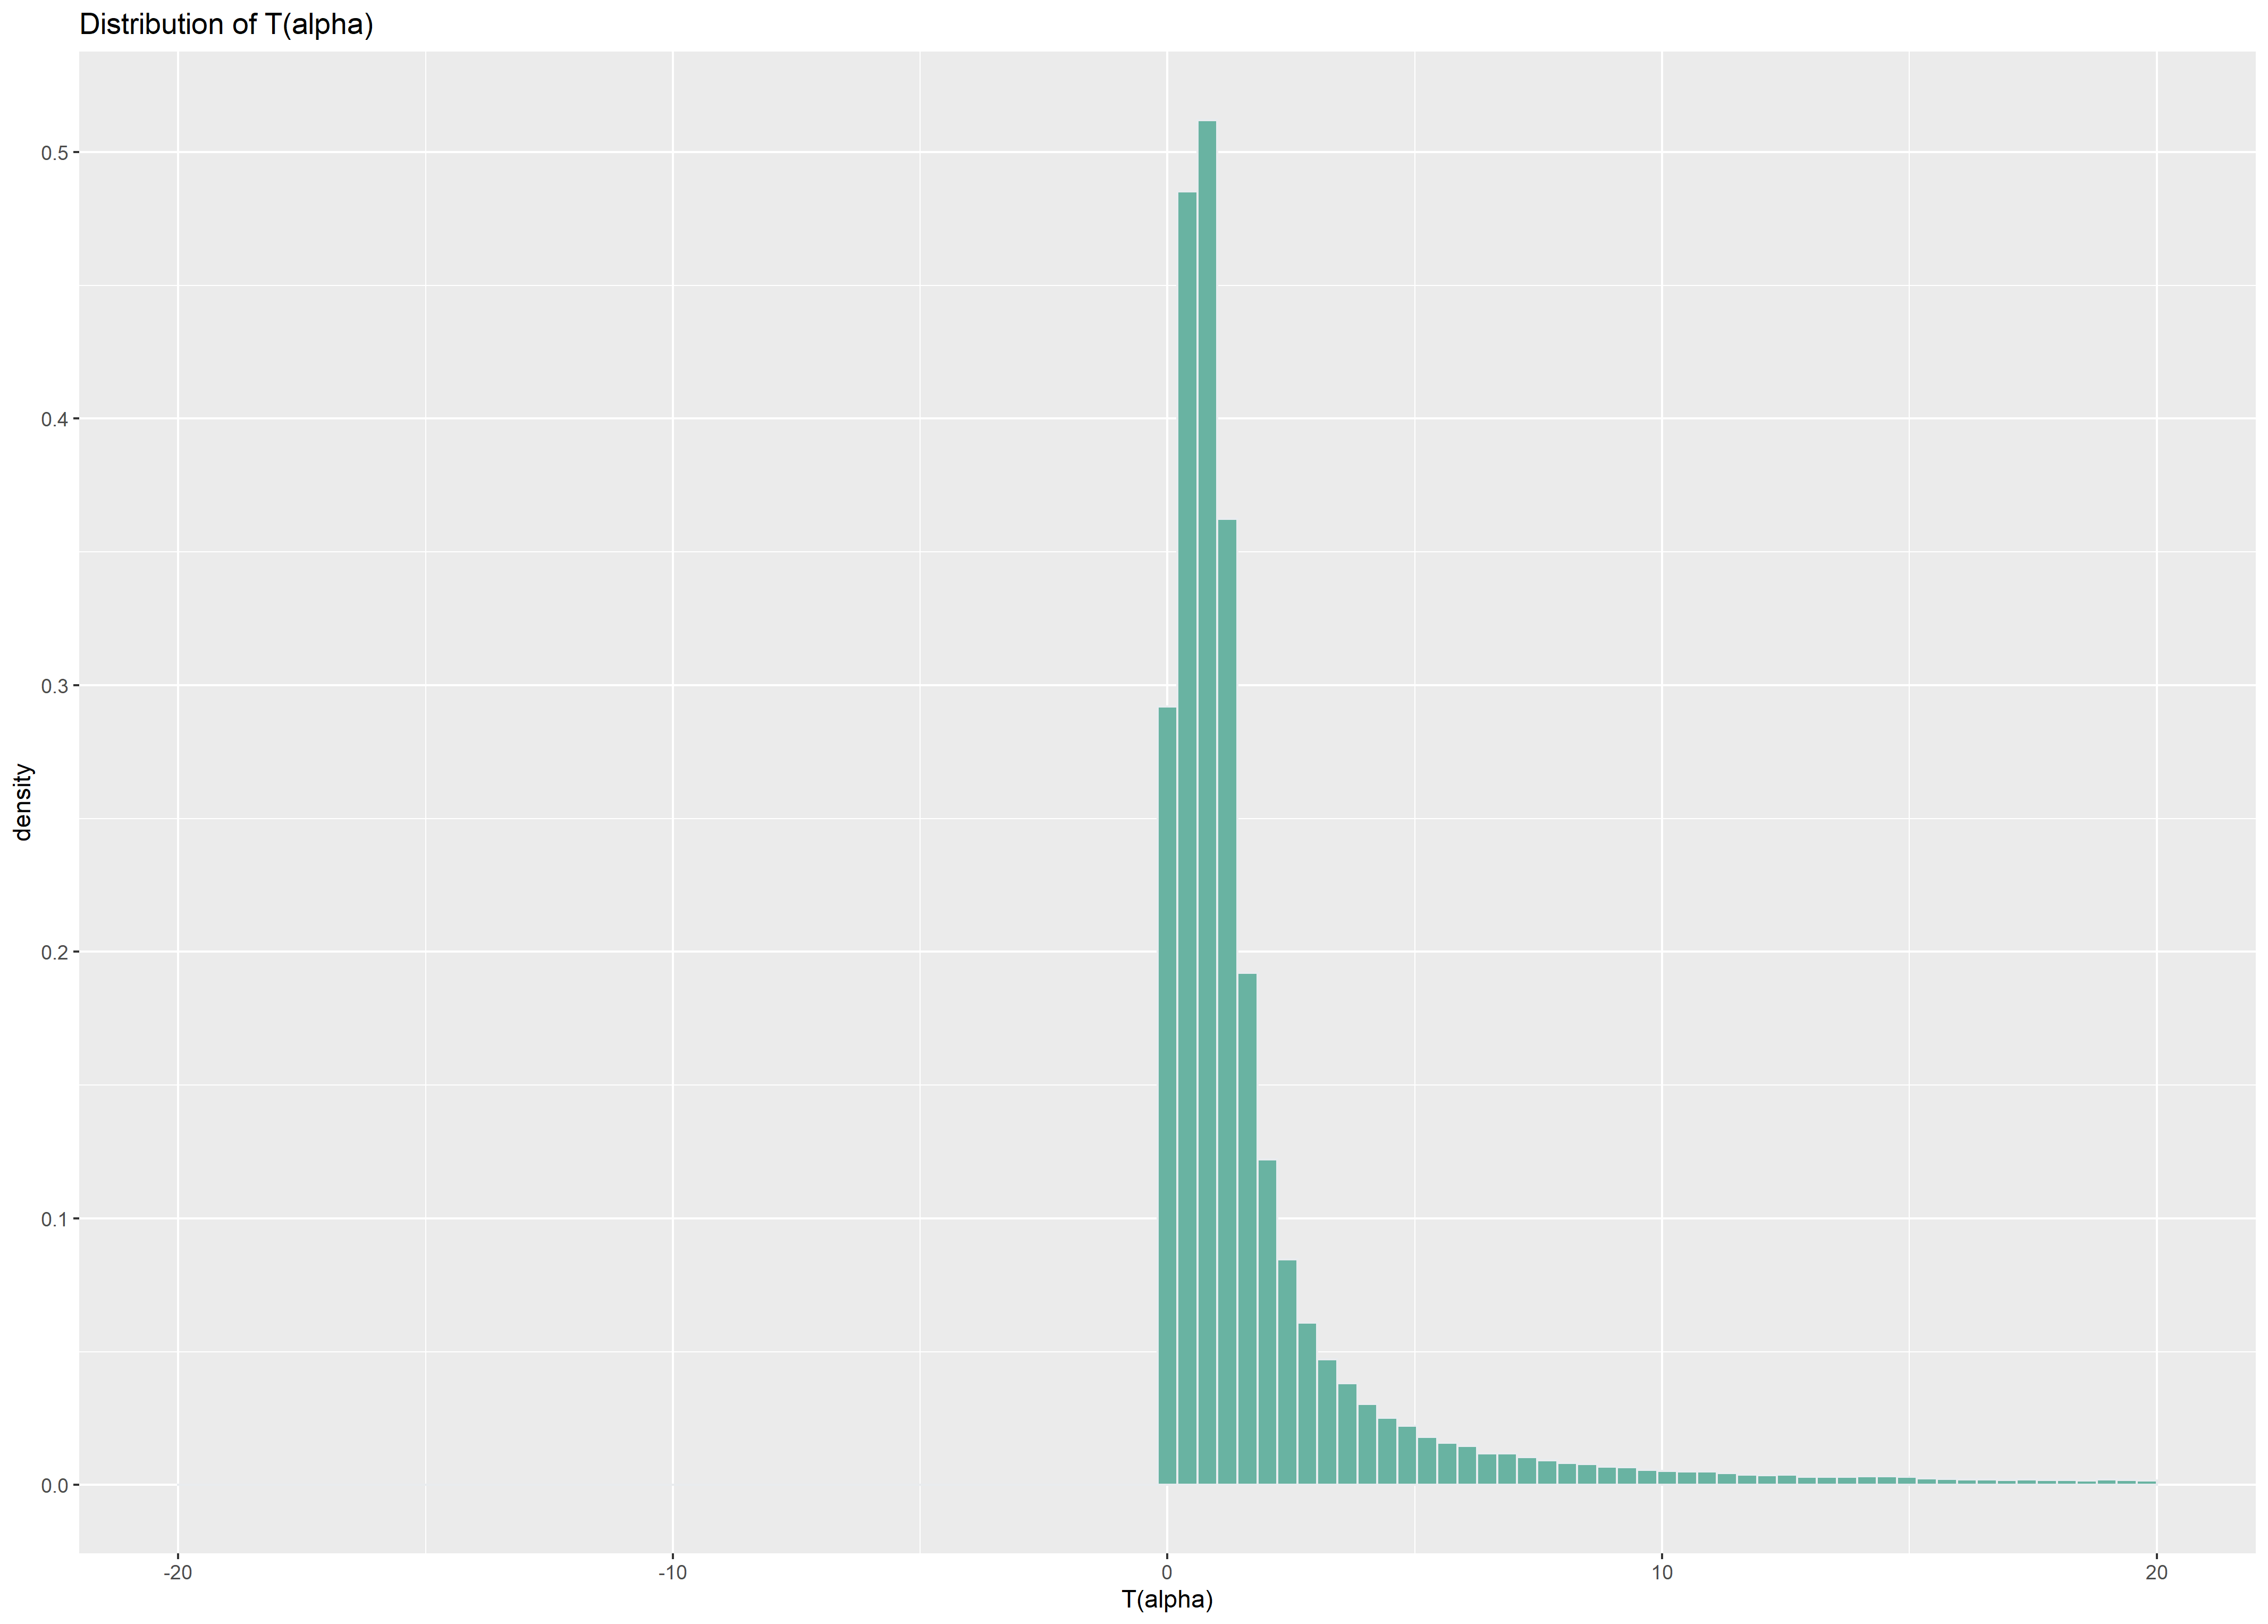
\includegraphics[width=\textwidth]{Figures/HSprior1.png}
     \end{subfigure}
     \hfill
     \begin{subfigure}[b]{0.49\textwidth}
         \centering
         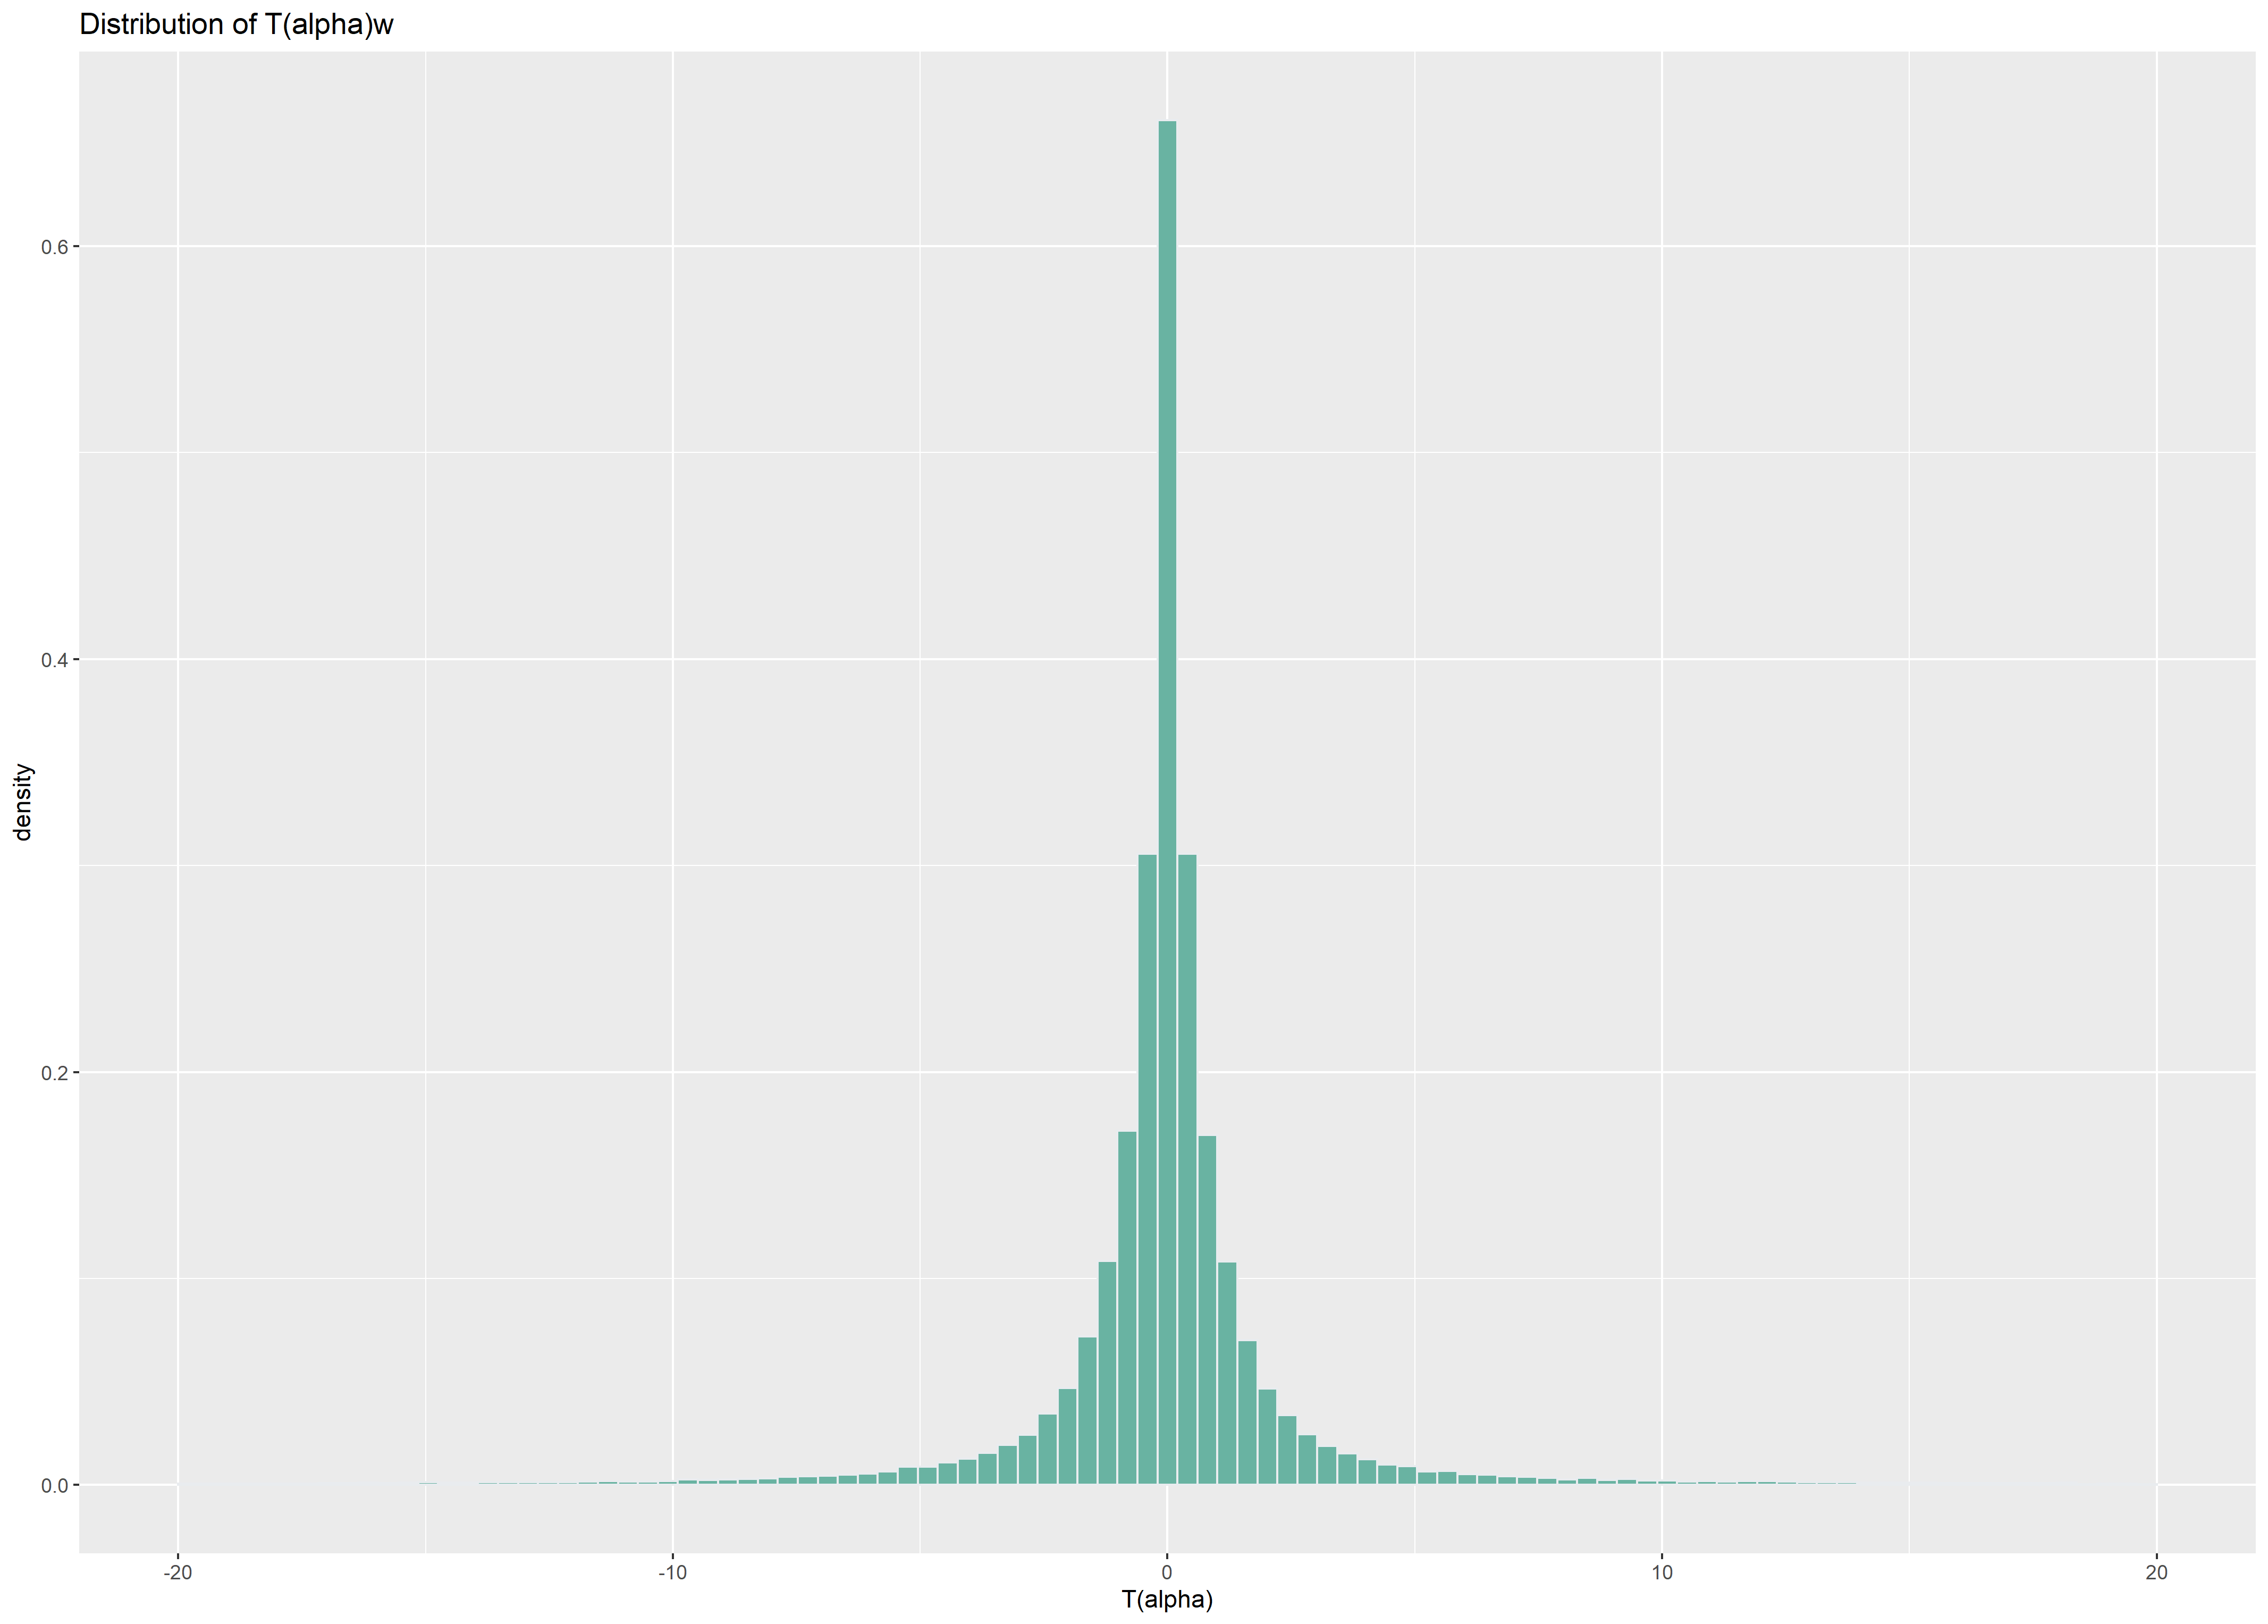
\includegraphics[width=\textwidth]{Figures/HSprior2.png}
     \end{subfigure}
     \hfill
     \begin{subfigure}[b]{0.49\textwidth}
         \centering
         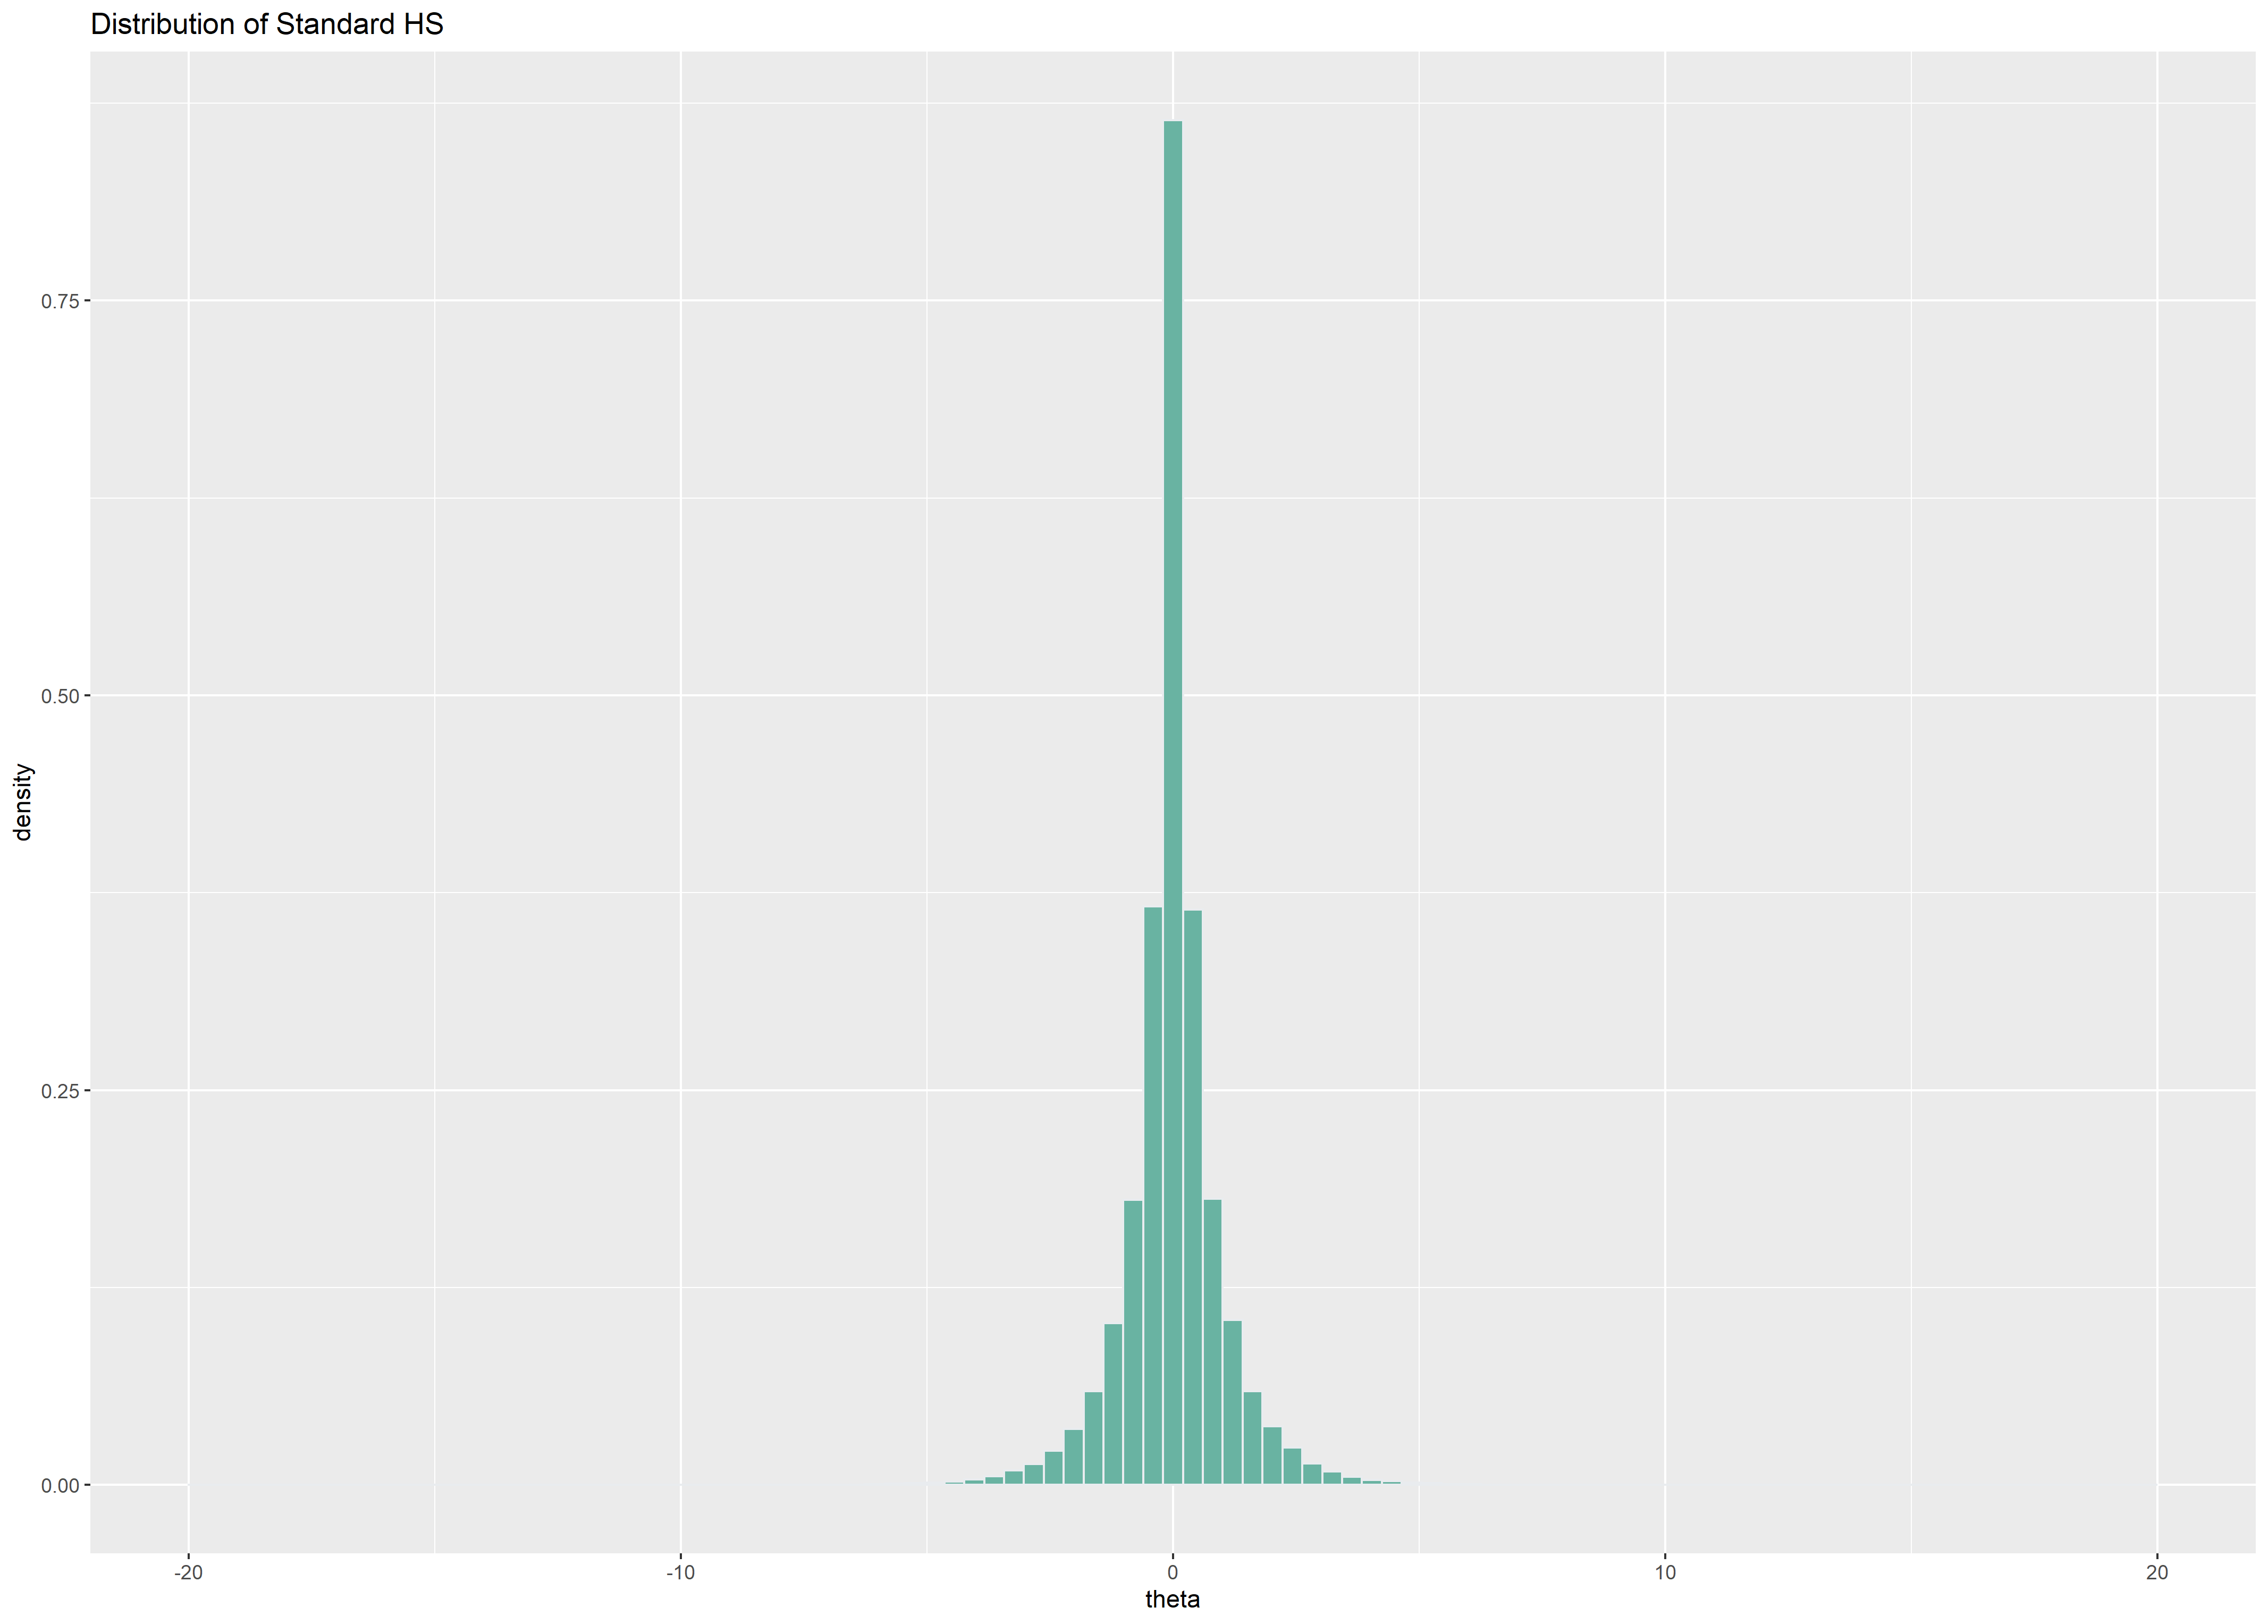
\includegraphics[width=\textwidth]{Figures/HSprior3.png}
     \end{subfigure}
        \caption{Histogram of $T(\alpha)$, $T(\alpha)w$, and the standard Horseshoe prior.}
        \label{fig:HS_prior}
\end{figure}

    In order to generalize horseshoe priors, as $\lambda_1$ indicates the tail behavior of the current neuronized prior, we add two more polynomial terms with lower exponents to the exponential activation function:
    \begin{align}
        T(t)=exp(\lambda_1 sign(t)t^2+\lambda_2 t+\lambda_3)
    \end{align}
    By numerically calculation, when $T(t)=exp(0.5 sign(t)t^2+0.733 t$, the neuronized prior approximate horseshoe prior well and $T(t)=exp(0.5 t^2-1.27t+0.29)$ approximate to standard Cauchy priors\cite{shin2021neuronized}. However, the generalized activation function for Cauchy will change to $T(t)=exp(\lambda_1 t^2+\lambda_2 t+\lambda_3)$ since this activation function will have stronger shrinkage effects for weak signals.
    
    Under this circumstance, the activation function solve the challenge that the corresponding MCMC algorithm can't achieve to geometric ergodicity under horseshoe prior, which is a heavy tail prior\cite{k1996the}. The MCMC procedure can achieve convergence more efficiently with the activation function, because the tail is stable in this case. 
   



\section{Managing Neuronized Priors }

\subsection{Find the Activation Function to Match a Given Prior}
In order to find an activation function $T(t)$ for the neuronized prior that discussed in section 3, the author introduce a family of $T(t)$, $T_\phi$, and then find the $\phi$ which could minimize the distance between the result neuronized prior and the target distribution $\pi(\theta)$. To enhance flexibility, the function space spanned by a class of B-spline basis function $B(t)$, B is a vector of $K$ dimension rational space where $\phi \in R^K$ . Consequently, $T_\phi(t)=B(t)\phi$.

The essay use neuronized horseshoe prior as an example, whose activation function is $T(t)=exp(\lambda_1 sign(t)t^2+\lambda_2 t+\lambda_3)$. In this case, $\phi = {\lambda_1,\lambda_2,\lambda_3}$. The class of activation function for horseshoe now become:
    \begin{align}
        T_\zeta(t) = exp(\lambda_1 sign(t)t^2+\lambda_2 t+\lambda_3)+B(t)\phi\\
        \zeta=\{\lambda_1,\phi\}
    \end{align}
As the determinant parameter of prior's tail behavior, $\lambda_1$ can be found to match the tail of the horseshoe prior base on the inequality property: For $\kappa > 0, c_1, c_2$ are some  positive constants, there exist: 
\begin{align}
    c_1(log|\theta|)^{-\frac{1}{2}}|\theta|^{(-1-\frac{1}{2\lambda_1})(1+\kappa})\leq\pi(\theta)\leq c_2(log|\theta|)^{-\frac{1}{2}}|\theta|^{(-1-\frac{1}{2\lambda_1})(1+\kappa})
\end{align}
After $\lambda_1$ is fixes, we generate a large number (S) of samples from $\Tilde{\theta_i}_{\zeta,i}=T_{\zeta,\phi}(\alpha_i-\alpha_0)\omega_i$ and $\theta_i\sim \pi(\theta), i = 1, 2,..., S$. Then by using a search algorithm to find $zeta$ to minimize $\sum_{i=1}^S |\Tilde{\theta_\zeta}^{(i)}-\theta^{(i)}|$\cite{s1983optimization}, where $\theta_\zeta^{(i)},\theta^{(i)}$ are the $i$th largest number of the generated samples.

\subsection{Choosing Hyper-Parameters}
There are two hyper-parameter that need to be determined: the global shrinkage parameter $\tau_\omega^2$ and the bias parameter $\alpha_0$.
As for the value of $\alpha_0$, there are several situation:
\begin{itemize}
    \item For continuous neuronized prior,$\alpha_0$ is set to the default value 0.
    \item For discrete Spsl prior, where $P(T(\alpha_j - \alpha_0) = 0|\alpha_0)=\Phi(\alpha_0)$. As the author stated for the discrete Spsl prior, a hyper-prior can be imposed on $\alpha_0$ so the the sparsity level is determined by the data set.
    \item Sampling $\alpha_0$ on other parameter in Gibbs sampling and RWMH algorithm is highly inefficient due to the high correlation of its posterior with that of other parameters.
\end{itemize}
When choosing value for $\tau_\omega^2$:
\begin{itemize}
    \item When $E (T^2(\alpha))$ is bounded, the value of $\tau_\omega^2$ need to reflect the signal strength in the data. However, a theoretical justified selection for $\tau_\omega^2$ has not been found.
    \item When $E (T^2(\alpha))$ doesn't bound such as horseshoe and Cauchy, we first find a shrinkage factor $\kappa_j$: $E_j (\kappa_0) = min{0.01,0.1 \times n/p}$, which determine the shrinkage level of $\theta_j$. Then we calculate $\tau_\omega^2$ by $$\tau_\omega^2=\frac{1-\kappa_j}{\kappa T^2(\alpha_j)}$$
\end{itemize}


\section{Sampling and Optimization With Neuronized Priors}

\subsection{MCMC Sampling with Neuronized Priors}

Under the linear regression model mentioned previously, the joint posterior distribution of the parameters follows the form of Equation \eqref{eq:post_joint}. Therefore, the full conditions can be written as follows. The conditional posterior distribution of $\bm{w}$. given other parameters is a Gaussian distribution,
\begin{equation} \label{eq:w_condi}
    \bm{w} | \bm{y}, \bm{\alpha}, \sigma^2, \tau_w^2 \sim N(\tilde{\mu}, \sigma^2 \tilde{\Sigma}),
\end{equation}
where $\tilde{\Sigma} = (D_\alpha X^T X D_\alpha + \sigma^2 \tau_w^{-2} I)^{-1}$, and $\tilde{\mu} = \tilde{\Sigma} D_\alpha X^T \bm{y}$, and $D_\alpha$ is defined as in Section \ref{sec:neu_def}. However, when the number of coefficients $p$ is large relative to the number of observations $n$, the computational complexity of solving $(D_\alpha X^T X D_\alpha + \sigma^2 \tau_w^{-2} I)^{-1}$ is highly expensive. \citet{shin2021neuronized} adopts the fast sampling procedure proposed in \citet{bhattacharya2016fast}, which reduces the complexity from $O(p^3)$ to $O(n^2p)$.

Because $w_j$ and $\alpha_j$ are highly correlated a posteriori, the algorithm draw samples from the posterior through the following scheme. For $j=1,\dots, p$, we draw sample $\alpha_j$ conditional on $\bm{\alpha}_{-j}$ and $\bm{w}$, that is, $\alpha_j^* \sim \pi(\alpha_j| \bm{y}, \bm{w}_{-j}, \bm{\alpha}_{-j})$ by a RWMH algorithm, based on the log-target function,
\begin{equation} \label{eq:log-target}
    - \log (v_j) / 2 - \alpha_j^2 /2 + v_j m_j^2 / (2\sigma^2),
\end{equation}
where $v_j = X^T_j X_j T(\alpha_j - \alpha_0) + \sigma^2 / \tau_w^2$, and $m_j = \vr^T X_j T(\alpha_j - \alpha_0)/v_j$. And then sample $w_j$ from $\pi(w_j| \bm{y}, \bm{\alpha_j}, \alpha_j^*)$, conditional on other parameters. 
\begin{equation} \label{eq:w_j_sample}
    w_j | \vy, \valpha_{-j},\alpha_j, \vw_{-j}, \sigma^2, \tau_w^2 \sim N(m_j, \sigma^2 v_j^{-1})
\end{equation} 
%Here $N(\alpha_j^{(t)}, 2^2)$ is used as the proposal distribution. 
For continuous neuronized priors, $\alpha_0$ is set to be 0 and for neuronized SpSL, a hyper parameter is imposed on $\alpha_0$ which is discussed in the next section. We implemented this algorithm with the help of the NPrior package included in \citet{shin2021neuronized}, and conducted simulation and real data examples in later sections. The detailed algorithm is shown in Algorithm \ref{alg:neu_MCMC}.

\begin{algorithm}[H]
\caption{A general MCMC algorithm for neuronized priors} \label{alg:neu_MCMC}
\begin{algorithmic}
\Require Initialization of $\valpha,\alpha_0, \vw, \sigma^2$.
\State Sample $\vw$ conditional on $\vy, \valpha, \sigma^2$ from Equation \eqref{eq:w_condi}.
\For {$i = 1,\dots, N$}
\State Set $\vr = \vy - X\vtheta(\valpha,\vw)$.
\For {$j = 1,\dots, p$}
\State Update $\vr = \vr + X_jT(\alpha_j-\alpha_0) w_j$.
\For {$irep=1,\dots,N$}
\State Sample $\alpha_j$ from $\alpha_j | \vy, \valpha_{-j}, \vw_{-j} ,\sigma^2, \tau_w^2$ using a RWMH step with Equation \eqref{eq:log-target}.
\State Sample $w_j$ from $w_j | \vy, \valpha_{-j},\alpha_j, \vw_{-j}, \sigma^2, \tau_w^2 $ with Equation \eqref{eq:w_j_sample}.
\EndFor
\State Update $\vr = \vr - X_jT(\alpha_j-\alpha_0) w_j$.
\EndFor
\State Sample $\sigma^2$ from $\sigma^2 | \vy, \valpha, \vw, \tau_w^2$.
\State Sample $\delta$ based on the method described in Section \ref{sec:samp_alpha0}.
\EndFor
\end{algorithmic}
\end{algorithm}

\subsection{Sample $\alpha_0$ efficiently} \label{sec:samp_alpha0}

Because of the high correlation between $\alpha_0$ and the $\alpha_j$’s, a naive MH approach in which $\alpha_0$ is updated by a MH step conditioned on $\valpha$ is highly inefficient. Therefore, \citet{shin2021neuronized} adopts a group-move via the generalized Gibbs sampling formulation proposed in \cite{liu2000generalised} which updates $\valpha$ and $\alpha_0$ simultaneously by a common shift $\delta \in \mathbb{R}$. Specifically, $(\valpha,\alpha_0)$ is updated in the way that
$$ (\valpha, \alpha_0) \rightarrow (\valpha + \delta \bm{1}, \alpha_0 + \delta),$$
where $\delta$ is sampled from $g(\delta) \propto \pi^*(\valpha + \delta \bm{1}, \alpha_0 + \delta)$, and $\pi^*(\valpha, \alpha_0)$ is the conditional posterior density for $\valpha$ and $\alpha_0$. 

When $a_0 = b_0 = 1$ in the prior, $g(\delta) = N((\valpha^T\valpha + \alpha_0)/(p+1) , (p+1)^{-1})$. Otherwise, an extra approximation step is needed. The algorithm in \citep{shin2021neuronized} uses a multiple-try MH independence sampler (MTM-IS) to sample $\delta$. It proposes multiple candidates $\delta_i$'s drawn independently from a proposal distribution and then chooses one from them with probability proportional to their importance weights.

\subsection{Computational advantage of neuronized discrete SpSL} \label{sec:neu_dis_spsl_com}

The paper \citep{shin2021neuronized} shows that a fully collapsed and a half collapsed Gibbs sampler can be applied to efficiently sample from the posterior with the standard discrete SpSL priors. However, both of the methods are mot feasible when the continuous parameters cannot be analytically integrate out. It demonstrates that the neuronized priors are computationally efficient while achieving the same effect as the standard discrete SpSL priors, even if the marginals cannot be derived analytically. As is shown in the proposition in the paper, with a ReLU activation function in the neuronized prior, the conditional distribution $\pi(\alpha_j|\vy, \vw_{(-j)}, \valpha_{(-j)})$ is a mixture of two truncated Gaussians and therefore can be sampled exactly.

Another advantage of using the ReLU activation function is that when sampling $\vw$, the conditional posterior distribution can be decomposed as a product of independent Gaussian densities so that the numerical inversion of matrix to compute $\tilde{\Sigma}$ in Equation \eqref{eq:w_condi} can be avoided.

\subsection{A Scalable Algorithm for Finding Posterior Modes}

For large dataset, the computation of MCMC algorithm may not be practical so that we may consider optimization-based algorithms. Several optimization methods have been proposed to conduct the posterior inference with the SpSL priors. For example, EMVS \citep{rovckova2014emvs} and SSLASSO \citep{rovckova2018spike} are two optimization procedures for the Bayesian SpSL variable selection problem.

\citet{shin2021neuronized} proposes a coordinate-ascent algorithm for neuronized (CAAN) priors which finds the MAP estimator. To reduce the chance of being trapped in a local optimum, CAAN uses a warm start strategy by initializing the hyper-parameter leading to a weak shrinkage and increasing the strength of shrinkage gradually. 

The algorithm uses a temperature scheme with temperatures $t_k$ such that $t_0 \leq \cdots \leq t_{2L+1}$. At each temperature $t_k$, the coordinate ascent iterations are conducted $M$ times. The CAAN algorithm updates the value of $\alpha_j$ by optimizing it when fixing other parameters $\bm{\alpha}_{-j}$ and $\bm{w}$. This optimization is easily feasible because the log posterior with respect to $\alpha_j$ is a simple linear combination of a quadratic function and a function of $T(\alpha_j-\alpha_0)$. And $\bm{w}$ is updated taking the advantage of conjugacy. To get rid of trapping in a local optima, a random noise $\xi \sim \exp (1)$ is added in the first $L$ levels of temperature scheme. By default, we set $M=20$, $L=10$, $N=20$, $t_k = (3-2k/L)^2$ for $k= 1, \dots L$, and $ t_{L+1} = \cdots = t_{2L}$. Detailed algorithm is provided in Algorithm \ref{alg:caan} . We implemented this algorithm and conducted simulation studies using it in later sections.

\begin{algorithm}[H]
\caption{The coordinate-ascent algorithm for neuronized prior (CAAN)} \label{alg:caan}
\begin{algorithmic}
\Require Initialization of $\valpha,\alpha_0, \vw, \sigma^2$.
\State Set a candidate set of temperature, $\{t_{(1)}, \dots, t_{(2L+1)}\}$.
\For {$l = 1,\dots, 2L+1$}
\State Set $t = t_{(l)}$.
\State Set $\vr = \vy - X\vtheta(\valpha,\vw)$.
\For {$irep=1,\dots,M$}
\For {$j = 1,\dots, p$}
\State Update $\vr = \vr + X_j T(\alpha_j - \alpha_0)w_j$.
\State Update $\alpha_j$ by optimizing the log marginalized posterior in Equation \eqref{eq:log-target} with respect to $\alpha_j$.
\State Update $w_j$ from $w_j | \vy, \valpha_{-j},\alpha_j, \vw_{-j}, \sigma^2, \tau_w^2 $ with Equation \eqref{eq:w_j_sample}.
\State Update $\vr = \vr - X_jT(\alpha_j-\alpha_0) w_j$.
\EndFor
\State Every $N$ iterations,
\State  Update $\sigma^2 = (\normtwo{\vy-X\vtheta(\valpha,\vw)}^2/t + 2b_1)/\{n+2a_1+2\}$.
\If{$l \leq L$}
    \State Set $\sigma^2 = \sigma^2 + \xi$, where $\xi \sim \exp(1)$.
\EndIf
\State  Update $\alpha_0 = \{\sum_{j=1}^p 1(\alpha_j > \alpha_0) + a_0 -1\}/ (p+b_0 -2).$
\EndFor
\EndFor
\end{algorithmic}
\end{algorithm}


\subsection{Comparison With Other Posterior Optimization Procedures}

We conduct simulation to compare the performance of the proposed CAAN and other optimization methods finding the MAP, parallel to what the paper did. We evaluate the property of the CAAN algorithm \citep{shin2021neuronized} and the EMVS \citep{rovckova2014emvs}, which evaluates the MAP estimator Based on an EM formulation. Two metrics are investigated in the study, the mean-squared error (MSE) and the extended Bayesian information criterion (EBIC), which is, 
$$ \text{EBIC} = \text{BIC} + \zeta |\bm{k}| \log p,$$
where $\bm{k}$ is the set of selected variables, $\zeta$ is a tuning parameter (here, $\zeta = 1$), and BIC is the Bayesian information criterion.

We generate synthetic data by setting the error variance $\sigma^2 = 1$, and the first 10 elements in the coefficient vector to be randomly 2 or -2, and the rest 0. For EBIC, we use $\nu_1 = 100$ and $\nu_0^{-1}$ takes value from $(1,1000)$. Values of EBIC and log-MSE are evaluated as iteration increases.

Figure \ref{fig:Opt_comparison} shows the optimization paths of EMVS and CAAN. We can see from the results that the optimization paths of EMVS quickly converged to some sub-optimal models, corresponding to different solutions when started with different random initializations. Although both procedures failed to provide consistent results when initialized with different starting configurations, CAAN was more stable than EMVS.

\begin{figure}[tp]
     \centering
     \begin{subfigure}[b]{0.45\textwidth}
         \centering
         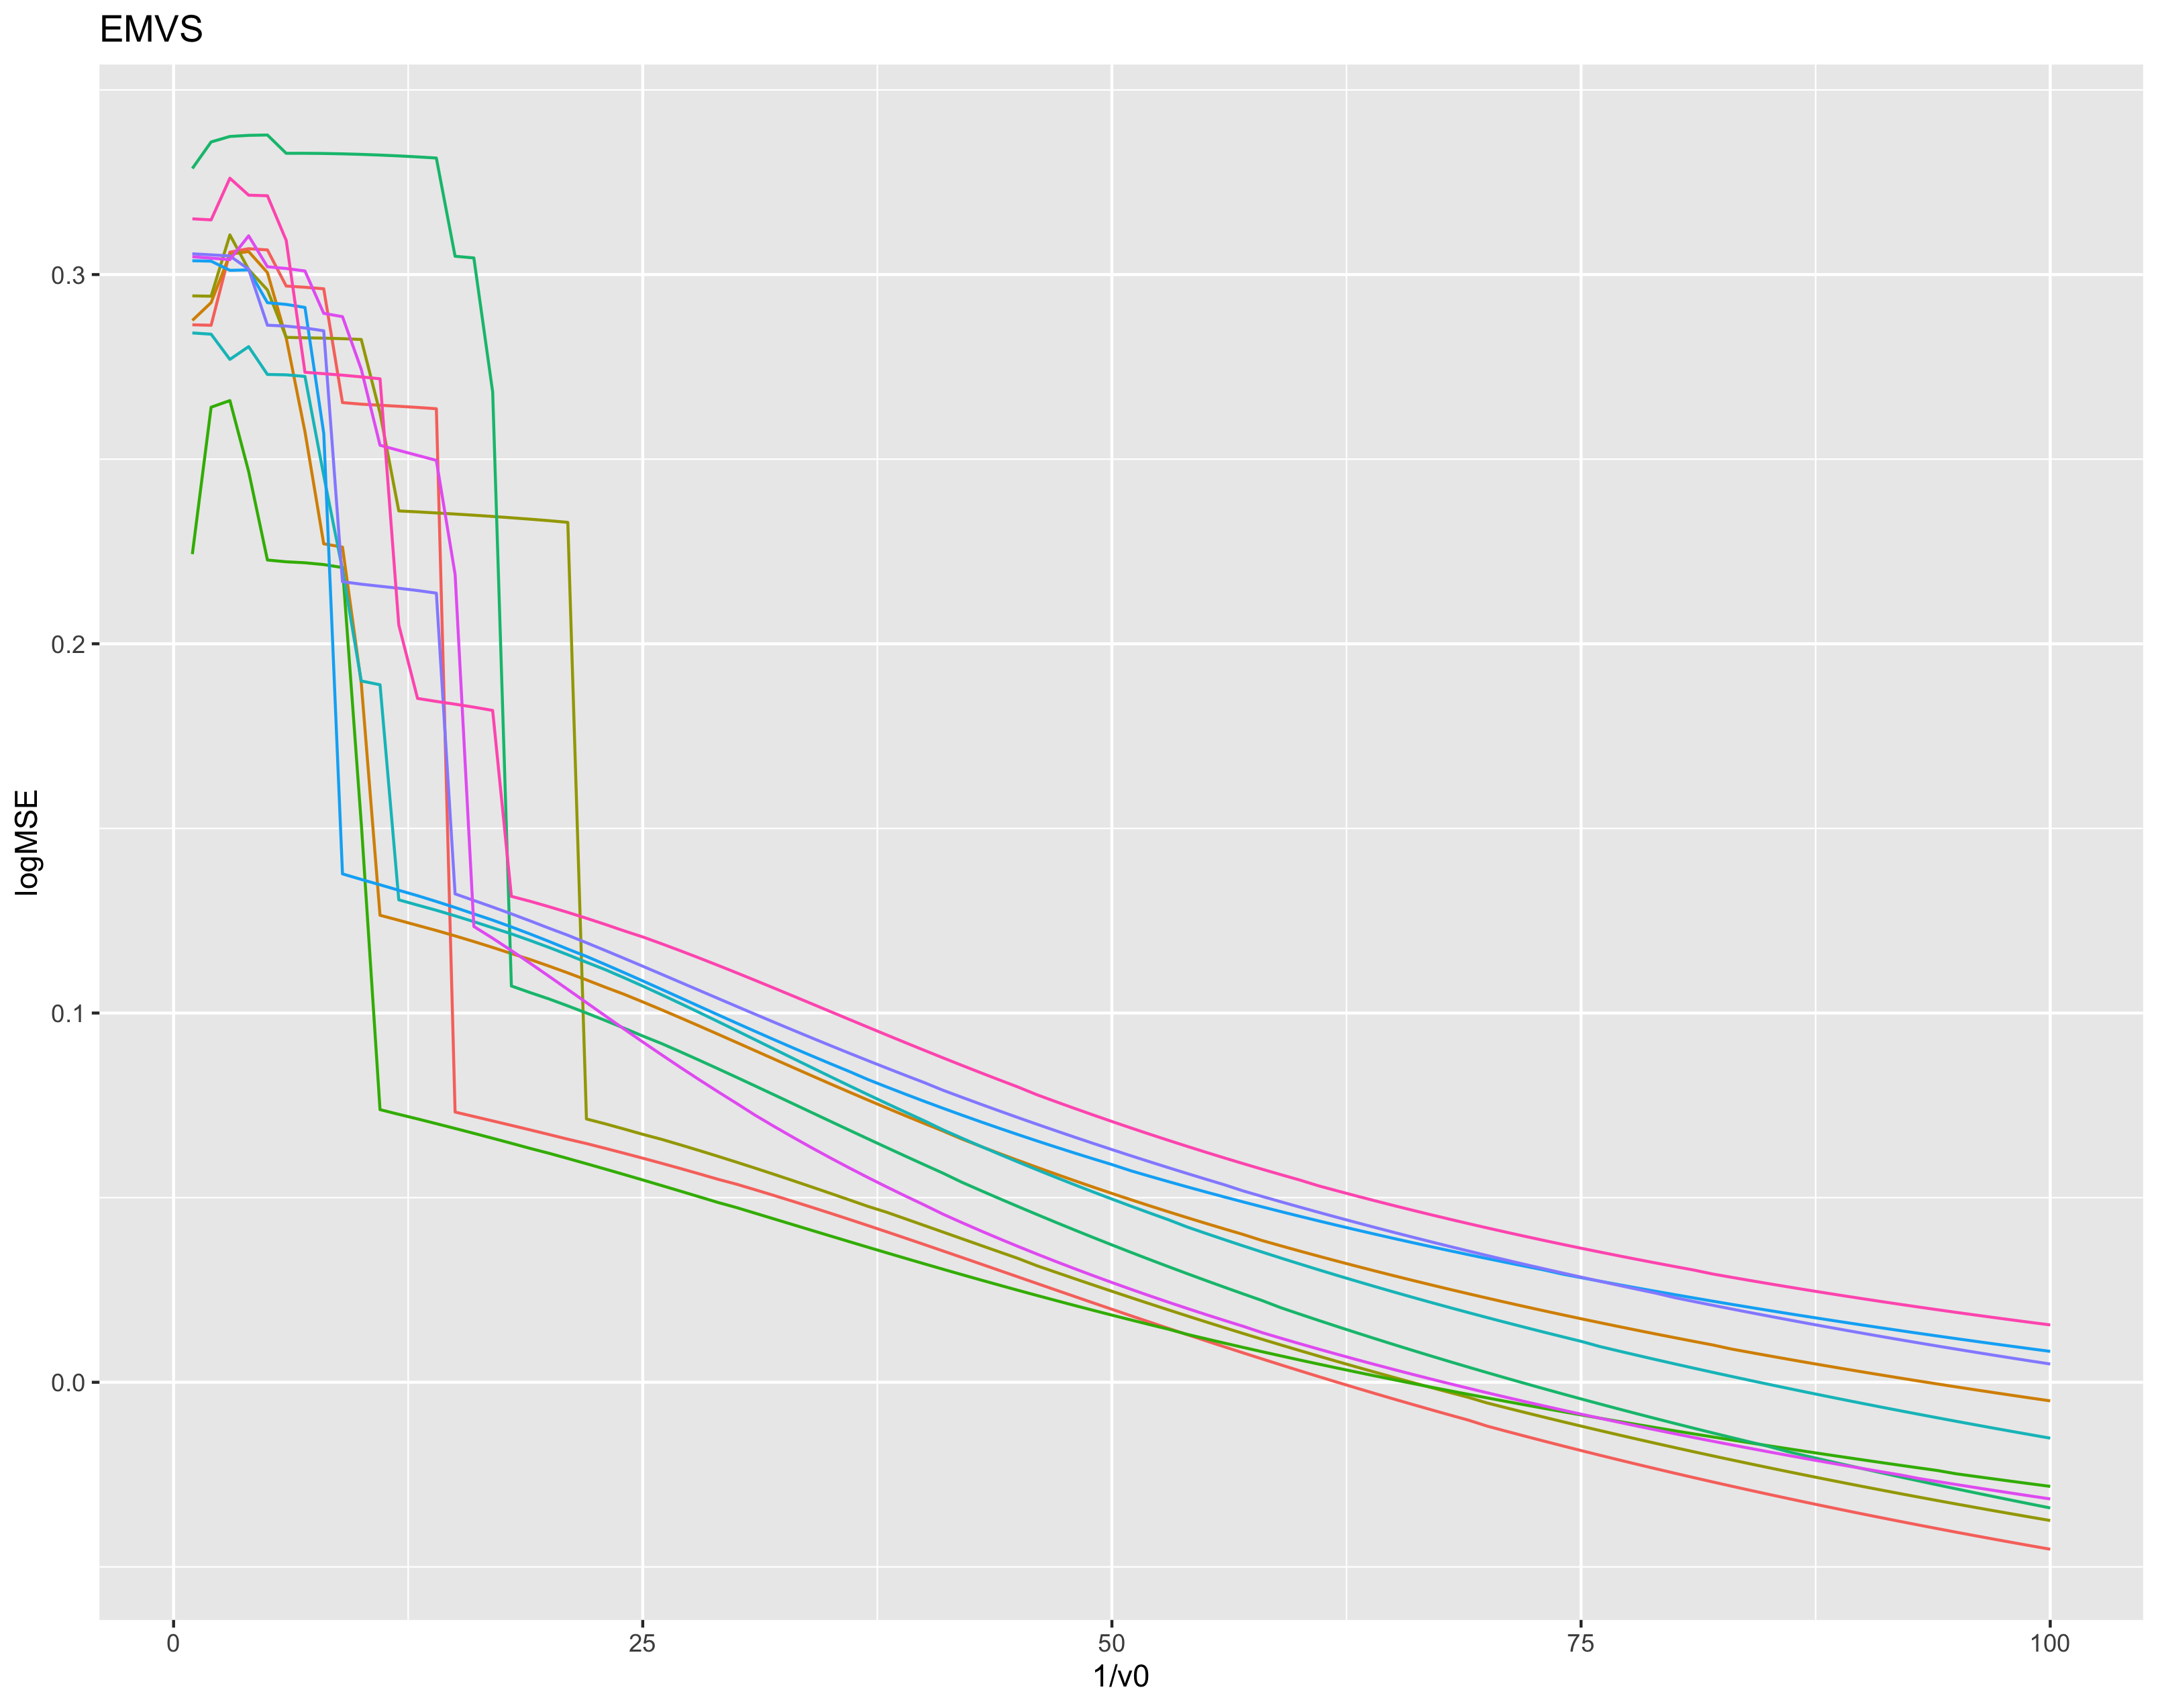
\includegraphics[width=\textwidth]{Figures/EMVS_MSE.png}
     \end{subfigure}
     \hfill
     \begin{subfigure}[b]{0.45\textwidth}
         \centering
         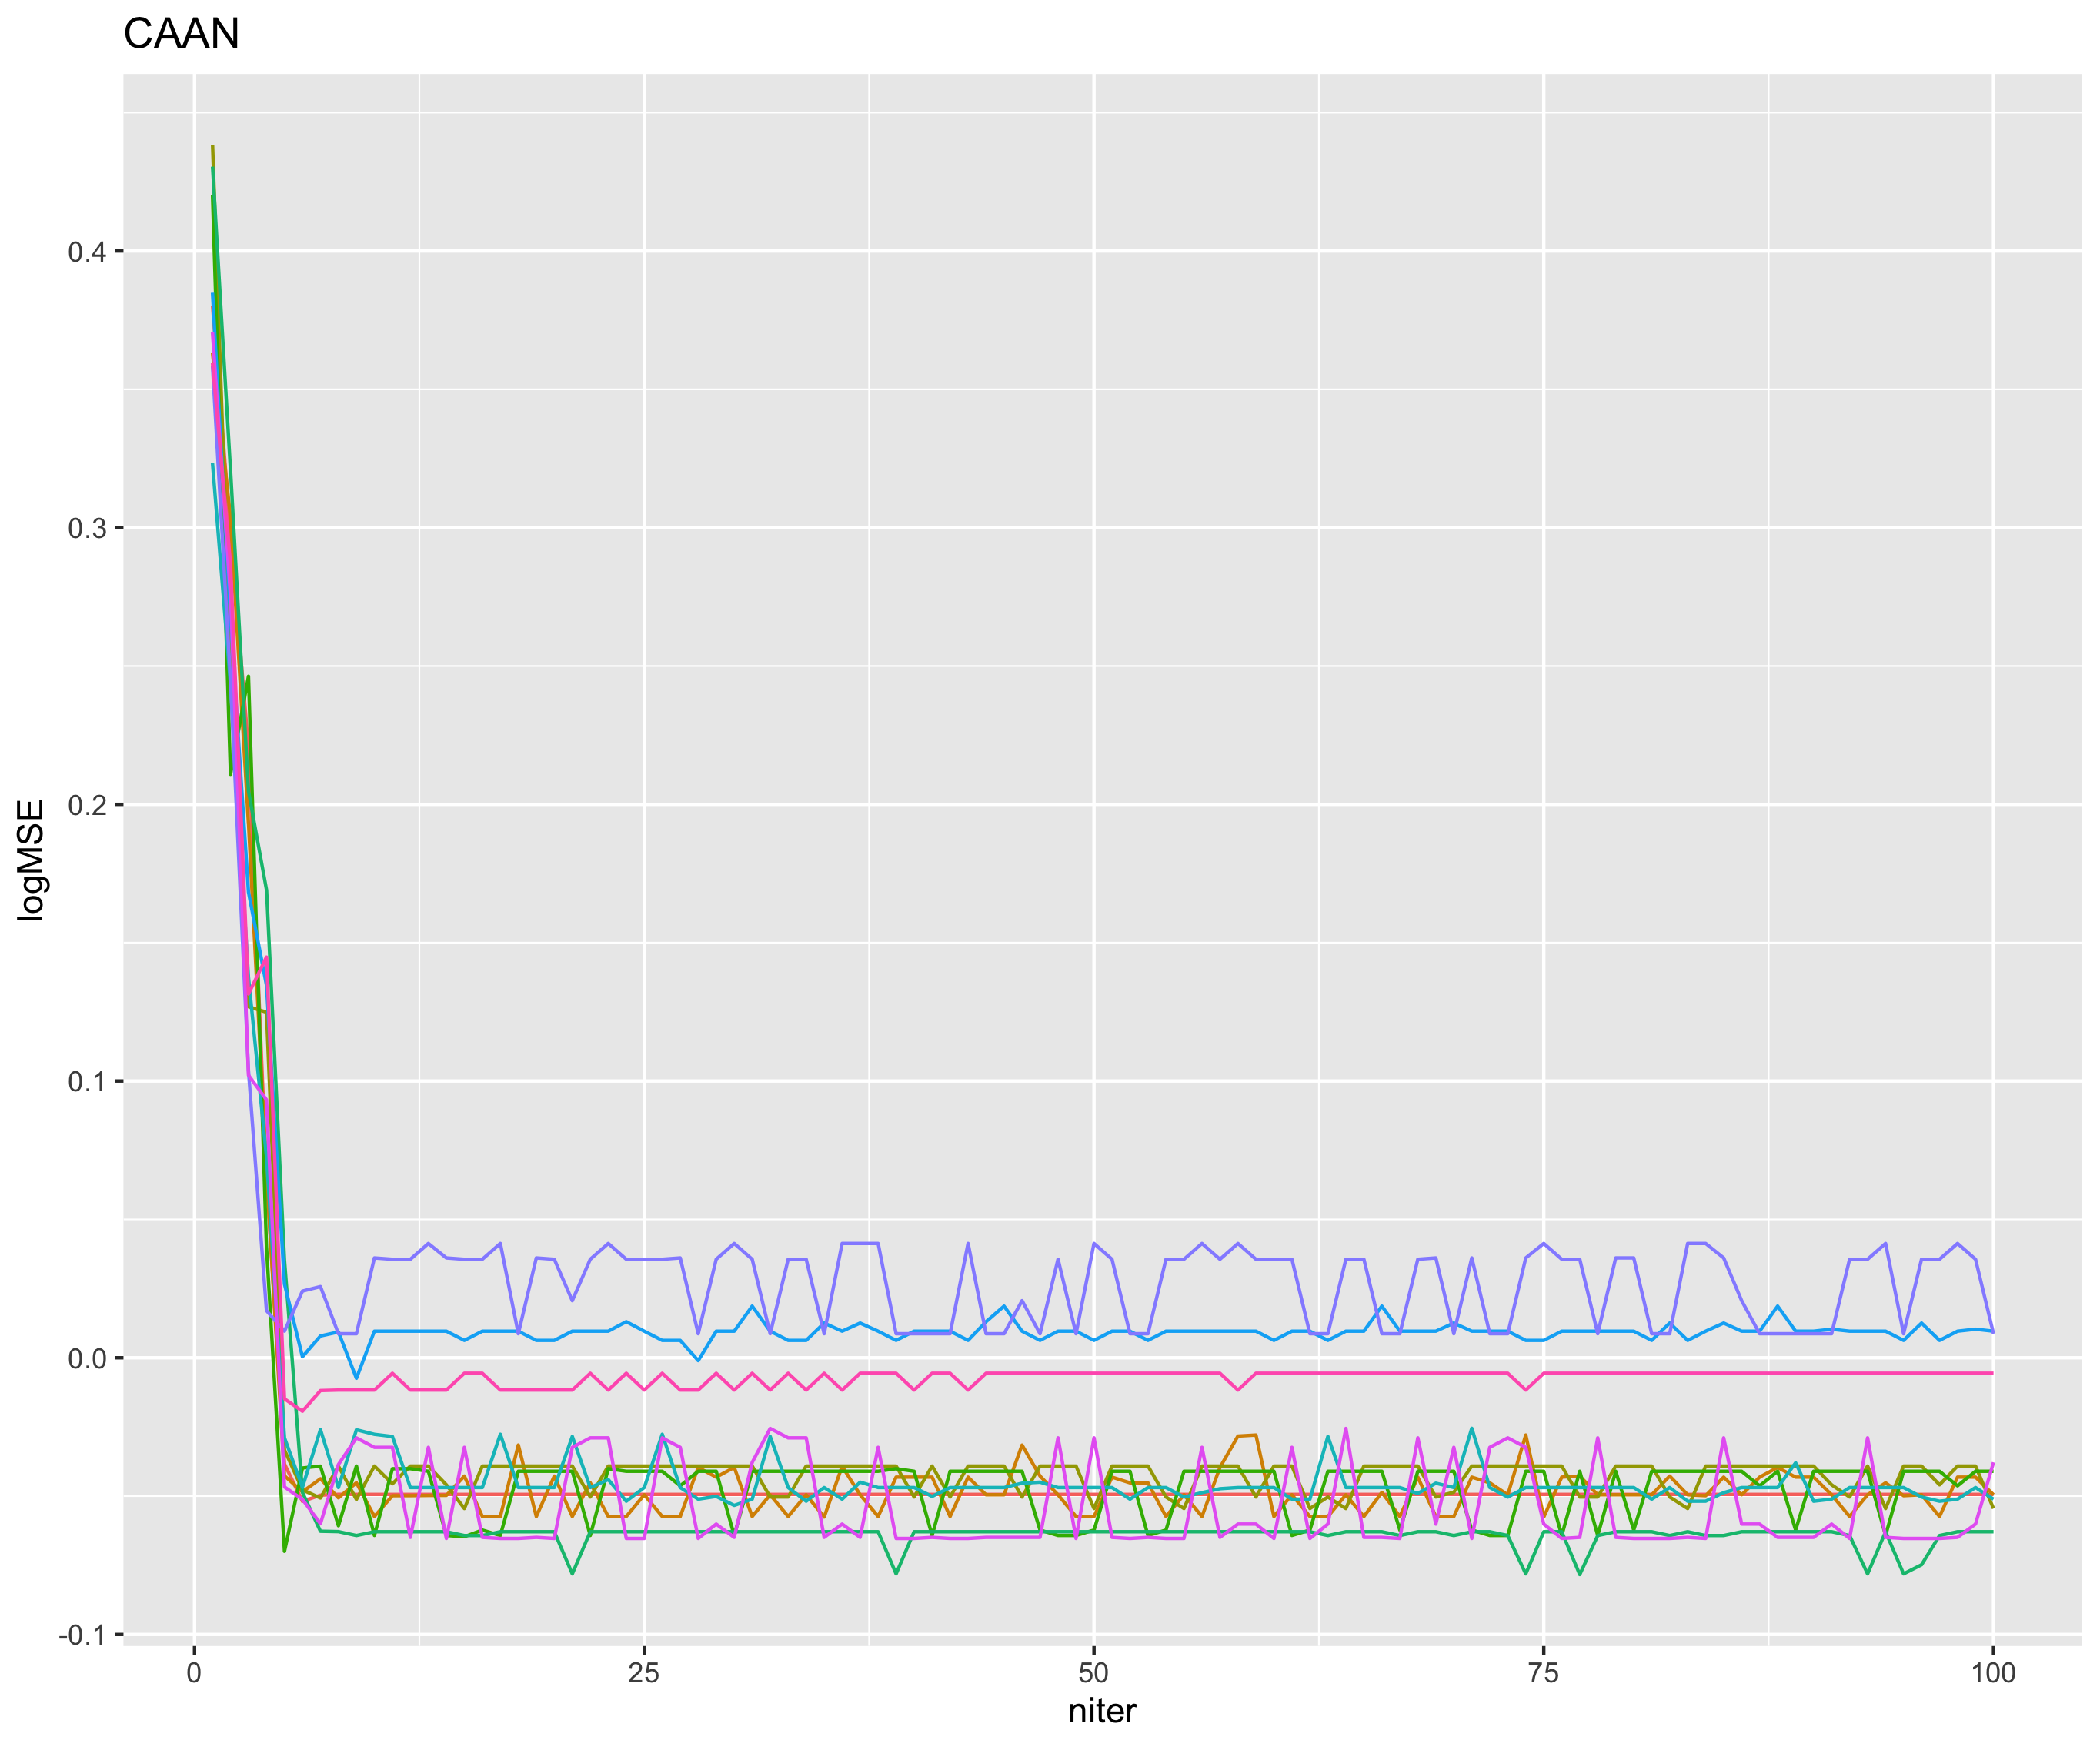
\includegraphics[width=\textwidth]{Figures/CAAN_MSE.png}
     \end{subfigure}
     \hfill
     \begin{subfigure}[b]{0.45\textwidth}
         \centering
         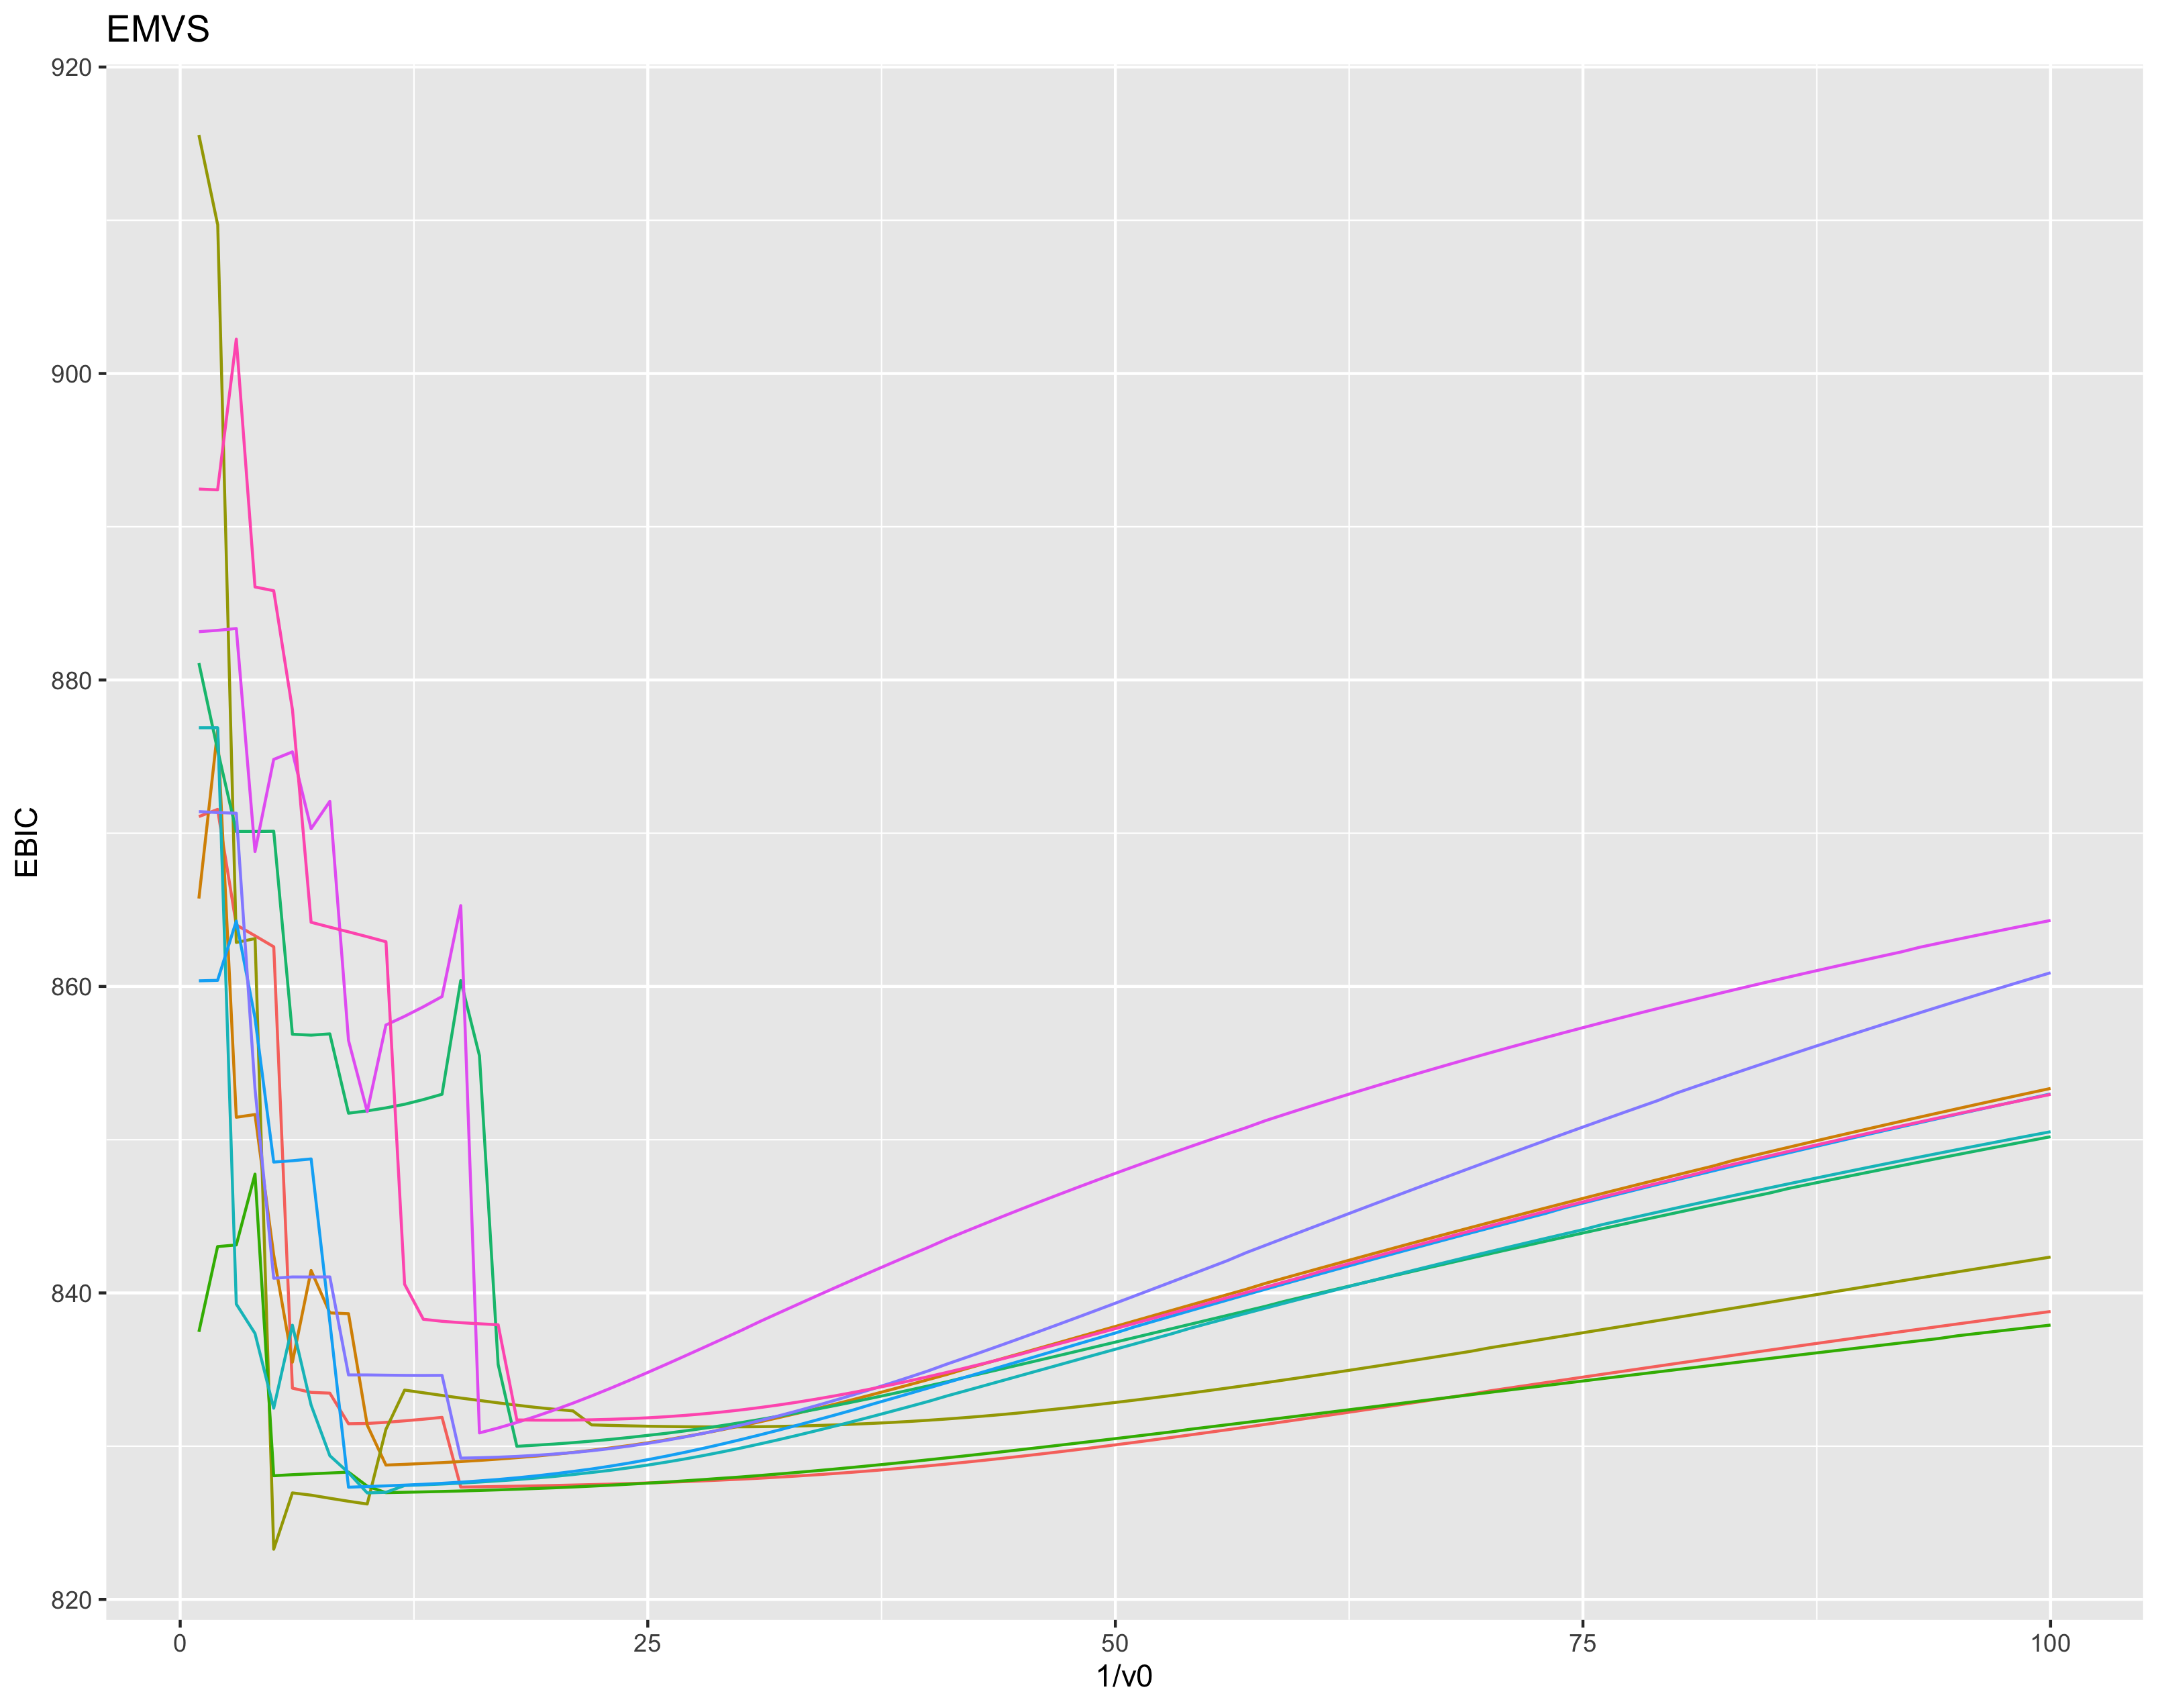
\includegraphics[width=\textwidth]{Figures/EMVS_EBIC.png}
     \end{subfigure}
     \hfill
     \begin{subfigure}[b]{0.45\textwidth}
         \centering
         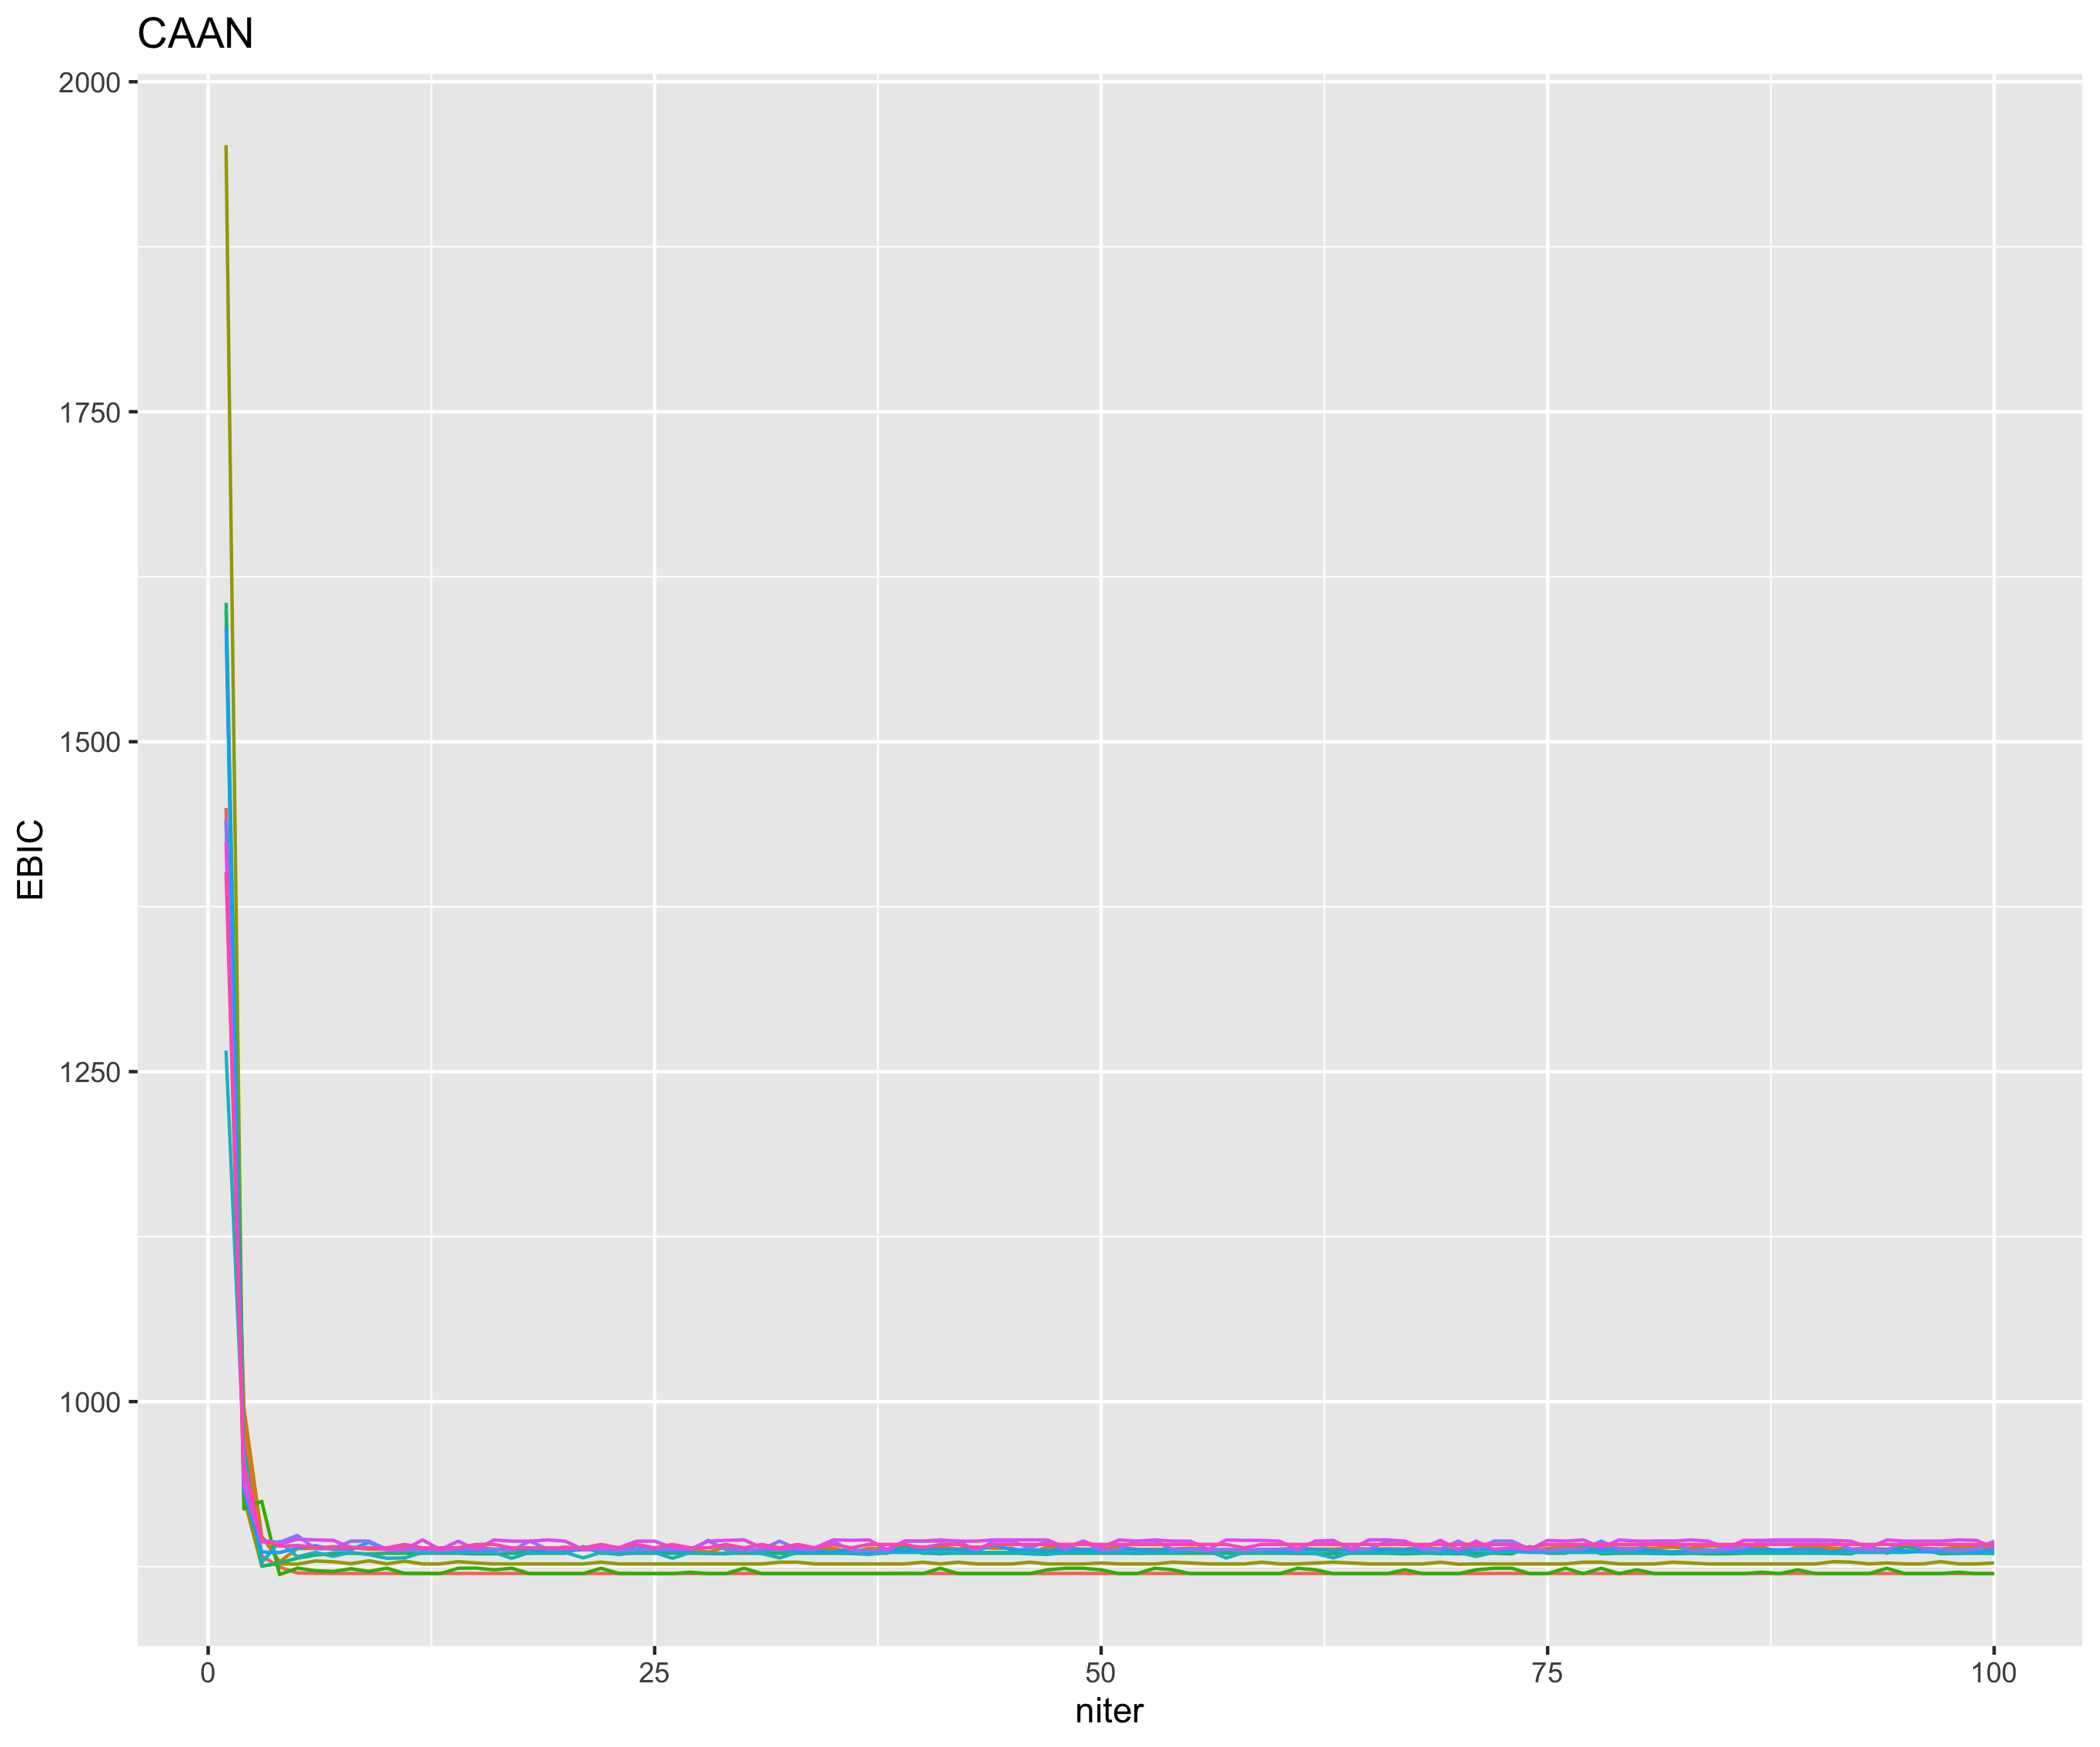
\includegraphics[width=\textwidth]{Figures/CAAN_EBIC.png}
     \end{subfigure}
        \caption{Trace plots of the log-MSE (top row) and EBIC (bottom row) paths from 10 different initial points for the EMVA and the CAAN optimization algorithms, based on a synthetic dataset generated (n = 120 and p = 200) with the true model 10. }
        \label{fig:Opt_comparison}
\end{figure}


\newpage
\section{Simulation and Real data examples}

\subsection{Simulation Settings}

We generate synthetic data to conduct simulation studies under the linear regression model. We compare the effect of some standard priors including the Bayesian LASSO, the horseshoe and the discrete SpSL with their neuronized counterparts. The optimization-based algorithms EMVS, SSLASSO and CAAN are also included in comparison. We implemented the proposed algorithms in \citet{shin2021neuronized} and a few R packages are used including Nprior, EMVS and SSLASSO. The notations of the methods for priors in comparison are as follows,
\begin{itemize}[itemsep=0pt]
    \item[-] SpSL-G: Standard discrete SpSL prior, $\pi_0(\theta) = \delta_0(\theta)$, $\pi_1(\theta) = \text{Gaussian}(\theta)$.
    \item[-] N-SpSL-L(Exact): The neuronized SpSL prior implemented via the exact Gibbs sampler as in Section \ref{sec:neu_dis_spsl_com}.
    \item[-] N-SpSL-L(RW): The neuronized SpSL prior with a Laplace-like slab via Algorithm \ref{alg:neu_MCMC} using the RWMH to update $\alpha$.
    \item[-] N-SpSL-C(RW): The neuronized SpSL prior with a Cauchy slab via Algorithm \ref{alg:neu_MCMC} using the RWMH to update $\alpha$.
    \item[-] HS: The Horseshoe prior.
    \item[-] N-HS(RW): The neuronized Horseshoe prior via Algorithm \ref{alg:neu_MCMC}.
    \item[-] BL: The Bayesian LASSO prior.
    \item[-] N-BL(RW): The neuronized Bayesian LASSO prior via Algorithm \ref{alg:neu_MCMC}.
    \item[-] N-SpSL(MAP): The neuronized SpSL using the CAAN optimization.
    \item[-] N-BL(MAP): The neuronized Bayesian LASSO using the CAAN optimization.
    \item[-] EMVS, SSLASSO : EMVS and SSLASSO.
    \item[-] LASSO(CV): LASSO with cross validation.
\end{itemize}


Note that the default $\tau_w$ is set to be 1 if not specified. We use $\nu_1 = 10$ for EMVS and $\lambda_1 = 0.1$ for SSLASSO.
As is conducted in \citet{shin2021neuronized}, for neuronized priors sampled by MCMC, Bayesian averaging is used for estimation and prediction. 

The Median probability model (MPM) is used to do variable selection, which picks variables with estimated posterior inclusion
probabilities greater than 0.5, i.e. variables that appear in at least half of the visited models. For neuronized priors, we consider selecting the variable $j$ when
$$1-\frac{1}{1+ T(\alpha_j-\alpha_0)^2} > 0.5.$$

\citet{shin2021neuronized} uses a half-collapsed sampling strategy to implement the inference with the SpSL prior to achieve high efficiency. Since no detailed algorithm is provided in the paper, it is hard to figure out and implement in a short time. We use the orthogonal data augmentation method proposed in \citet{ghosh2011rao} instead to implement models with SpSL prior.

We generated the synthetic data by considering a Toeplitz design. The covariates $X_i,\; i=1,\dots,n$ are generated from $N(0,\Sigma)$, where $\Sigma = (\sigma_{lk})$ with $\sigma_{lk} = 0.7^{|l-k|}$ for $l,k = 1,\dots p$. We generated two scenarios of low-dimentional cases, in which $n=200$, $p=50$, and $n=400$, $p=100$, respectively. The number of non-zero coefficients is $p/10$ and they take values from $\pm 0.2$. And another two high-dimentional cases are considered, with $n=100$, $p=300$, and $n=150$, $p=1000$. First five coefficients are non-zero and they are randomly $\{\pm 0.4, \pm 0.45, \pm 0.5, \pm 0.55, \pm 0.6\}$. The error variance is set to be $\sigma^2=1$ for all scenarios.


\subsection{Metrics}
\label{sim_metrics}
Shin et al. use three metrics to measure correct sparsity of posterior distributions.

First is mean squared error(MSE) of the predicted coefficient vector from the true data generating parameter vector.
MSE for multivariate parameter estimation is calculated as follows.
\begin{enumerate}
    \item Create estimate $\hat{\boldsymbol{\beta}}$ from sparse prior or equivalent neuronization.
    \item Compute the squared Euclidean distance from the estimate to the true data generating parameter vector.
    \label{mse_computation}
    \item Repeat for $n$ dataset instantiations.
    \item Calculate the average squared Euclidean distatnce across all $n$ distances.
\end{enumerate}

Second is cosine similarity.
This is calculated in a similar manner as MSE above, except that before step \ref{mse_computation} each estimate is also normalized by it's own euclidean distance from the origin.

%mcc
Next is the Mathews correlation coefficient (MCC).
This measure is used to determine how correlated each sparse prior is with predicting non-negative coefficients in the true data generating parameter vector.
The MCC is defined in terms of \textit{tp} (true positive predictions), \textit{fp} (false positive predictions), \textit{tn} (true negative predictions), and \textit{fn} (false negative predictions).
To clarify, false negatives are instances in which the inference (derived from a particular sparse prior) predicted a zero coefficient for a predictor, but the true coefficient was actually non-zero.

%fp
The FP metric, then, is simply the average number of times (over dataset instantiations) a coefficient in the full coefficient vector was estimated to be non-zero, when in fact the true scalar parameter was zero.

%ess
The final metric for the simulated dataset was effective sample size (ESS). 
It is intended to give an indication of the number of uncorrelated MCMC samples.
It is calculated as:
\begin{equation*}
    \frac{N}{1+2*\sum_t^\infty \rho(t)}
\end{equation*}
Where $N$ is the number of MCMC samples and $\rho(t)$ is lag-t autocorrelation.
\subsection{Simulation results}
\label{simulation_results}

Tables \ref{table:low1}, \ref{table:low2}, \ref{table:high1}, and \ref{table:high2} show the results of the simulation on the low dimensional and high dimensional settings. In general, the results are identical to the ones in the original paper. We can see from the results that no procedure clearly dominate others in all situations for all criteria. Bayesian averaging results generally have a better performance than the corresponding MAP estimator. And the Lasso-based procedures typically show the best estimation performance under the low-dimensional settings, but they tends to select a large number of false positives. For high dimensional scenarios, the SpSL based priors out performs other methods.

The tables also list the performances of optimization-based SpSL procedures including the CAAN, the EMVS, and the SSLasso. The results show that, overall, the CAAN and the SSLasso significantly outperformed the EMVS algorithms in terms of estimation and model selection.

% latex table generated in R 4.1.1 by xtable 1.8-4 package
% Mon Dec 13 12:24:12 2021
\begin{table}[ht]
\centering
\begin{tabular}{rlllll}
  \hline
 & MSE & Cos(Angle) & MCC & FP & ESS \\ 
  \hline
SpSL-G & 0.228(0.004) & 0.573 & 0.37(0.22) & 0.79 & 3020.3 \\ 
  N-SpSL-L(Exact) & 0.228(0.004) & 0.579 & 0.25(0.2) & 2.19 & 2922.7 \\ 
  N-SpSL-C(RW) & 0.223(0.004) & 0.547 & 0.23(0.24) & 0.17 & 2985.7 \\ 
  N-HS(RW) & 0.223(0.003) & 0.585 & 0.09(0.14) & 21.42 & 2994.4 \\ 
  HS & 0.270(0.004) & 0.44 & 0.18(0.07) & 3.79 & 1483.7\\ 
  BL &     0.324(0.013)&     0.494&     0.212(0.009)&    21.290&  2348.971\\
  N-BL(RW) & 0.328(0.006) & 0.586 & 0.06(0.15) & 10.61 & 2745.4 \\ 
  N-SpSL(MAP) & 0.197(0.007) & 0.551 & 0.46(0.2) & 2.1 &  \\ 
  N-BL(MAP) & 0.205(0.008) & 0.548 & 0.43(0.21) & 2.49 &  \\ 
  EMVS & 0.254(0.006) & 0.507 & 0.4(0.18) & 5.75 &  \\ 
  SSLASSO & 0.278(0.01) & 0.534 & 0.39(0.2) & 5.84 &  \\ 
  Lasso(CV) &0.145(.005)& 0.548 & 0.160(.009)& 6.03&\\
   \hline
\end{tabular}
\caption{Results for low-dimensional setting (n=200, p=50)} 
\label{table:low1}
\end{table}


% latex table generated in R 4.1.1 by xtable 1.8-4 package
% Mon Dec 13 14:32:12 2021
\begin{table}[ht]
\centering
\begin{tabular}{rlllll}
  \hline
 & MSE & Cos(Angle) & MCC & FP & ESS \\ 
  \hline
SpSL-G & 0.373(0.004) & 0.585 & 0.45(0.15) & 1.03 & 3018 \\ 
  N-SpSL-L(Exact) & 0.362(0.004) & 0.591 & 0.37(0.14) & 2.92 & 2997.8 \\ 
  N-SpSL-C(RW) & 0.378(0.004) & 0.557 & 0.31(0.13) & 0.18 & 3012.4 \\ 
  N-HS(RW) & 0.361(0.004) & 0.63 & 0.1(0.1) & 41.77 & 2978.2 \\ 
  HS & 0.344(0.004) & 0.68 & 0.21(0.14) & 2.83 & 1489.2\\
  BL &     0.344(0.010)&     0.624&     0.253(0.004)&    25.470&  2355.409\\
  N-BL(RW) & 0.472(0.005) & 0.691 & 0.18(0.11) & 21.17 & 2698 \\ 
  N-SpSL(MAP) & 0.265(0.008) & 0.667 & 0.61(0.16) & 2.64 &  \\ 
  N-BL(MAP) & 0.266(0.008) & 0.672 & 0.61(0.16) & 2.8 &  \\ 
  EMVS & 0.409(0.006) & 0.602 & 0.54(0.12) & 9.04 &  \\ 
  SSLASSO & 0.35(0.009) & 0.656 & 0.56(0.13) & 7.21 &  \\ 
  Lasso(CV) & 0.238(0.006)&     0.645&     0.194(0.007)&    12.820 &\\
   \hline
\end{tabular}
\caption{Results for low-dimensional setting (n=400, p=100)} 
\label{table:low2}
\end{table}


% latex table generated in R 4.1.1 by xtable 1.8-4 package
% Mon Dec 13 18:51:02 2021
\begin{table}[ht]
\centering
\begin{tabular}{rlllll}
  \hline
 & MSE & Cos(Angle) & MCC & FP & ESS \\ 
  \hline
SpSL-G & 1.468(0.061) & 0.675 & 0.31(0.15) & 13.97 & 2803.3 \\ 
  N-SpSL-L(Exact) & 1.182(0.021) & 0.625 & 0.24(0.16) & 6.7 & 2996.6 \\ 
  N-SpSL-C(RW) & 1.093(0.021) & 0.63 & 0.3(0.22) & 0.55 & 2875.1 \\ 
  N-HS(RW) & 1.387(0.023) & 0.634 & 0.05(0.05) & 143.59 & 2954.8 \\ 
  HS & 1.66(0.034) & 0.71 & 0.54(0.01) & 99.35 & 2563.2\\
  BL &     0.931(0.020)&     0.586&     0.073(0.003)&     4.210&  2395.840\\

  N-BL(RW) & 1.721(0.021) & 0.527 & 0.06(0.06) & 90.55 & 2860.3 \\ 
  N-SpSL(MAP) & 1.43(0.047) & 0.475 & 0.27(0.13) & 13.35 &  \\ 
  N-BL(MAP) & 1.436(0.049) & 0.482 & 0.26(0.13) & 13.28 &  \\ 
  EMVS & 1.588(0.02) & 0.318 & 0.28(0.1) & 21.13 &  \\ 
  SSLASSO & 0.994(0.033) & 0.526 & 0.4(0.21) & 8.14 &  \\ 
  Lasso(CV) &     0.896(0.022)&     0.579&     0.072(0.004)&    14.200&\\
   \hline
\end{tabular}
\caption{Results for high-dimensional setting (n=100, p=300)} 
\label{table:high1}
\end{table}


% latex table generated in R 4.1.1 by xtable 1.8-4 package
% Sun Dec 12 05:16:16 2021
\begin{table}[ht]
\centering
\begin{tabular}{rlllll}
  \hline
 & MSE & Cos(Angle) & MCC & FP & ESS \\ 
  \hline
SpSL-G & 2.921(0.154) & 0.538 & 0.13(0.13) & 245.52 & 223.3 \\ 
  N-SpSL-L(Exact) & 0.983(0.026) & 0.659 & 0.27(0.14) & 8.23 & 156.1 \\ 
  N-SpSL-C(RW) & 0.956(0.026) & 0.624 & 0.35(0.21) & 0.54 & 152.6 \\ 
  N-HS(RW) & 1.973(0.031) & 0.656 & 0.03(0.03) & 482.06 & 132.4 \\ 
  HS & 0.259(0.032) & 0.594 & 0.12(0.16) & 60.89 & 2678.1\\
  BL &     1.163(0.032)&     0.378&     0.238(0.016)&    13.610&   146.434\\
  N-BL(RW) & 1.828(0.023) & 0.51 & 0.13(0.03) & 312.13 & 132.4 \\ 
  N-SpSL(MAP) & 0.239(0.087) & 0.53 & 0.33(0.16) & 9.77 &  \\ 
  N-BL(MAP) & 0.272(0.094) & 0.494 & 0.29(0.13) & 12.82 &  \\ 
  EMVS & 1.32(0.01) & 0.242 & 0.74(0.17) & 0.08 &  \\ 
  SSLASSO & 1.063(0.037) & 0.496 & 0.36(0.19) & 12.2 &  \\ 
  Lasso(CV)&     0.869(0.023)&     0.626&     0.375(0.019)&    21.350& \\
   \hline
\end{tabular}
\caption{Results for high-dimensional setting (n=150, p=1000)} 
\label{table:high2}
\end{table}


\subsection{Real data examples}
To validate the results in \ref{simulation_results}, Shin et al. applied all procedures to two real-world datasets (described in Section \ref{real_world_datasets}).
Since the true data generating parameter is no longer known, evaluating each procedure was altered slightly from Section \ref{sim_metrics}.
These changes are described in Section \ref{real_world_eval}.
We then discuss our results as they relate to those reported by Shin et al. in Section \ref{real_world_discuss}

\subsubsection{Datasets}
\label{real_world_datasets}
The first dataset is the Boston Housing data. 
This dataset has $n=506$ datapoints that record information about distinct houses in the Boston area.
Shin et al. do not mention which version of this dataset they used, but we obtained it through the mlbench package available on CRAN.

This version has 14 features with the \textit{medv} (i.e. median value) feature being the target variable for regression.
Shin et al. mention they only used 10 of the other variables for regression, but neglect to mention which ones were used.
We therefore used all remaining 13 for our regression experiments on this dataset.

The second dataset used was the Bardet-Beidl syndrome dataset which contains $p=200$ features indicating gene expression information in $n=120$ rats.
Because this dataset has $p>n$ features, inference with most of the tested algorithms took longer than with the Boston Housing dataset.

\subsubsection{Evaluation}
\label{real_world_eval}
Shin et al. used three metrics to evaluate shrinkage prior performance on the datasets.

%mspe
The first is mean-squared \textit{predictive} error (MSPE).
This is similar to the MSE described above, but the squared error is taken with respect to the regression variable rather than the full coefficient vector. 
As such, the MSPE takes it's average over every predicted datapoint in the dataset.
This is in contrast to MSE which only measured the squared error between the one parameter vector estimate obtained from the posterior and the true vector.  
Since Shin et al. repeated their experiments 100 times, each MSPE estimate was averaged again.
% and the results are reported in Tables \ref{table:boston} and \ref{table:bardet}.

%cos angle
Shin et al. also used cosine angle as a metric in their real-world dataset experiments.
Similar to the MSE measure, the cosine similarity could no longer be made with respect to the coefficient vector.
If $\mathbf{y}$ is the dependent regression variable in the dataset and the $\mathbf{\hat{y}}$ is the prediction, then the cosine similarity used here in $\mathbf{y}^T \mathbf{\hat{y}}/(\Vert\mathbf{y}\Vert\cdot\Vert\mathbf{\hat{y}}\Vert)$.
This measure indicates the correlation between the prediciton and actual response variable

% model size
The final metric used is \textit{model size}.
This is simply the average number of non-zero coefficients chosen by each procedure. 
\subsubsection{Discussion}
\label{real_world_discuss}
The results for the experiments on the Boston Housing dataset can be found in Table \ref{table:boston} and the Bardet-Biedl experiments in Table \ref{table:bardet}.

% latex table generated in R 4.1.1 by xtable 1.8-4 package
% Mon Dec 13 13:12:50 2021
\begin{table}[ht]
\centering
\begin{tabular}{rlll}
  \hline
 & MSPE & Cos(Angle) & MS \\ 
  \hline
SpSL-G & 24.577(0.951) & 0.843 & 5.17 \\ 
  N-SpSL-L(Exact) & 24.246(0.995) & 0.846 & 8.52 \\ 
  N-SpSL-C(RW) & 24.397(1.005) & 0.846 & 5.24 \\ 
  N-HS(RW) & 24.493(0.962) & 0.844 & 7.74 \\ 
  HS & 24.377(1.23) & 0.843 & 7.764\\
  BL&     26.7(0.9)&     0.857&    12.260\\
  N-BL(RW) & 24.377(1.03) & 0.846 & 7.03 \\ 
  N-SpSL(MAP) & 23.977(0.987) & 0.845 & 7.68 \\ 
  N-BL(MAP) & 23.974(0.986) & 0.845 & 8.44 \\ 
  Lasso(CV) &     26.7(0.9)&     0.857&    12.260\\
   \hline
\end{tabular}
\caption{Results for Boston housing dataset} 
\label{table:boston}
\end{table}

In the Boston housing experiments there is a striking similarity in all neuronized procedures.
We hypothsise that this is due mainly to the similar optimization method that is used in each of them. 
It is also noteworthy that the model sizes of each neuronized implementation are substantially less than both the Bayesian Lasso (BL) and Lasso procedures.


% latex table generated in R 4.1.1 by xtable 1.8-4 package
% Mon Dec 13 19:36:36 2021
\begin{table}[ht]
\centering
\begin{tabular}{rlll}
  \hline
 & MSPE & Cos(Angle) & MS \\ 
  \hline
SpSL-G & 0.018(0.001) & 0.572 & 99.38 \\ 
  N-SpSL-L(Exact) & 0.049(0.003) & 0.674 & 110.12 \\ 
  N-SpSL-C(RW) & 0.026(0.002) & 0.645 & 1.81 \\ 
  N-HS(RW) & 0.017(0.001) & 0.698 & 98.13 \\ 
HS & 0.018(0.008) & 0.689 & 87.63\\
BL &     0.907(0.072)&     0.083&    30.080\\
  N-BL(RW) & 0.022(0.001) & 0.649 & 59.19 \\ 
  N-SpSL(MAP) & 0.735(0.064) & 0.589 & 1.93 \\ 
  N-BL(MAP) & 0.844(0.253) & 0.601 & 62.06 \\
  Lasso(CV) &     0.454(0.026)&     0.658&    32.010\\
   \hline
\end{tabular}
\caption{Results for Bardet-Biedl dataset} 
\label{table:bardet}
\end{table}

In the Bardet-Biedl experiments, however, there was a lot more variability in the model sizes induced by each procedure. 
This trend is matched in the MSPE for each procedure, which saw scores as low as .017 for the neuronized horseshoe prior, all the way to .907 for the Bayesian Lasso. 
The Bayesian Lasso, in particular, appeared to struggle with finding good regression coefficient estimates as evidenced by it's cosine angle of .089. 
Further study is needed to explain the behavior of the Baysian Lasso in this setting.


\section{Conclusion}

By replicating the experiments in Shin and Liu's essay\cite{shin2021neuronized}, it is found that there are still some differences between our experimental results for simulated and real data and the results given by the authors. However, while the same analysis program was used, the difference between the results for the real data is relatively small, while the difference between the results for the simulated data is large, which could indicate that the difference in the results may come from the difference between the simulated sample data set and the original work, while the data processing process itself is not too problematic.

From the results in the table, we can see that the neuronized prior usually has a smaller ESS than the original prior, which proves that the neuronizing operation can improve the efficiency of analyzing the data, and the difference is most obvious in horseshoe prior.

As in the Shin and Liu's essay, the MSE of lasso shows the best estimation performance, but the false positive is higher. By comparing MCC, we found that SpSL prior generally has a better model selection process in high dimensional settings, while horseshoe and its neuronized prior has a preferred result in low-dimensional setting.
%
\section{Chris Crabtree (My Own) - Contribution}
In terms of experments, I helped by implementing the Lasso and Baysian Lasso procedures. 
I also started on the SSLASSO procedure, but ran out of time. 
Additionally, I took charge of  navigating the evaluation produres for the experiments.
The original authors were quite terse in their descriptions and left several experimental settings ambiguous or underspecified.
I was tasked, then, with exploring several possible options for evaluation to see which type produced the results seen in the paper.

Since I made those contributions, I naturally was responsible for the bulk of the writing of the report w.r.t. the lasso procedures and the presentation of experimental results.
I also helped create the introductory slides for the video presentation.
\section{Yunshan Duan - Contribution}
Yunshan was for sure the MVP of the group. 
She implemented the majority of the algorithms and also wrote the largest chunks of the paper

\section{Lanxin Yang - Contribution}
Lanxin helped by implementing the Horseshoe prior and filling out large portions of the Standard Prior section of the report.
She was also responsible for the video editing.
\newpage
\bibliographystyle{plainnat}
\bibliography{refs}

\end{document} 
